% This template is borrowed from the Reed College LaTeX thesis template. Most of the work
% for the document class was done by Sam Noble (SN), as well as this
% template. Later comments etc. by Ben Salzberg (BTS). Additional
% restructuring and APA support by Jess Youngberg (JY).
% Your comments and suggestions are more than welcome; please email
% them to cus@reed.edu
%
% See http://web.reed.edu/cis/help/latex.html for help. There are a
% great bunch of help pages there, with notes on
% getting started, bibtex, etc. Go there and read it if you're not
% already familiar with LaTeX.
%
% Any line that starts with a percent symbol is a comment.
% They won't show up in the document, and are useful for notes
% to yourself and explaining commands.
% Commenting also removes a line from the document;
% very handy for troubleshooting problems. -BTS

% As far as I know, this follows the requirements laid out in
% the 2002-2003 Senior Handbook. Ask a librarian to check the
% document before binding. -SN

%%
%% Preamble
%%
% \documentclass{<something>} must begin each LaTeX document
\documentclass[12pt,twoside]{deuthesis}
% Packages are extensions to the basic LaTeX functions. Whatever you
% want to typeset, there is probably a package out there for it.
% Chemistry (chemtex), screenplays, you name it.
% Check out CTAN to see: http://www.ctan.org/
%%
\usepackage{graphicx,latexsym}
\usepackage{amsmath}
\usepackage{amssymb,amsthm}
\usepackage{longtable,booktabs,setspace}
\usepackage{chemarr} %% Useful for one reaction arrow, useless if you're not a chem major
\usepackage[hyphens]{url}
% Added by CII
\usepackage{hyperref}
\usepackage{lmodern}
\usepackage{float}
\floatplacement{figure}{H}
% End of CII addition
\usepackage{rotating}

% Next line commented out by CII
%%% \usepackage{natbib}
% Comment out the natbib line above and uncomment the following two lines to use the new
% biblatex-chicago style, for Chicago A. Also make some changes at the end where the
% bibliography is included.
%\usepackage{biblatex-chicago}
%\bibliography{thesis}


% Added by CII (Thanks, Hadley!)
% Use ref for internal links
\renewcommand{\hyperref}[2][???]{\autoref{#1}}
\def\chapterautorefname{Chapter}
\def\sectionautorefname{Section}
\def\subsectionautorefname{Subsection}
% End of CII addition

% Added by CII
\usepackage{caption}
\captionsetup{width=5in}
% End of CII addition

% \usepackage{times} % other fonts are available like times, bookman, charter, palatino

% Syntax highlighting #22
  \usepackage{color}
  \usepackage{fancyvrb}
  \newcommand{\VerbBar}{|}
  \newcommand{\VERB}{\Verb[commandchars=\\\{\}]}
  \DefineVerbatimEnvironment{Highlighting}{Verbatim}{commandchars=\\\{\}}
  % Add ',fontsize=\small' for more characters per line
  \usepackage{framed}
  \definecolor{shadecolor}{RGB}{248,248,248}
  \newenvironment{Shaded}{\begin{snugshade}}{\end{snugshade}}
  \newcommand{\AlertTok}[1]{\textcolor[rgb]{0.94,0.16,0.16}{#1}}
  \newcommand{\AnnotationTok}[1]{\textcolor[rgb]{0.56,0.35,0.01}{\textbf{\textit{#1}}}}
  \newcommand{\AttributeTok}[1]{\textcolor[rgb]{0.77,0.63,0.00}{#1}}
  \newcommand{\BaseNTok}[1]{\textcolor[rgb]{0.00,0.00,0.81}{#1}}
  \newcommand{\BuiltInTok}[1]{#1}
  \newcommand{\CharTok}[1]{\textcolor[rgb]{0.31,0.60,0.02}{#1}}
  \newcommand{\CommentTok}[1]{\textcolor[rgb]{0.56,0.35,0.01}{\textit{#1}}}
  \newcommand{\CommentVarTok}[1]{\textcolor[rgb]{0.56,0.35,0.01}{\textbf{\textit{#1}}}}
  \newcommand{\ConstantTok}[1]{\textcolor[rgb]{0.00,0.00,0.00}{#1}}
  \newcommand{\ControlFlowTok}[1]{\textcolor[rgb]{0.13,0.29,0.53}{\textbf{#1}}}
  \newcommand{\DataTypeTok}[1]{\textcolor[rgb]{0.13,0.29,0.53}{#1}}
  \newcommand{\DecValTok}[1]{\textcolor[rgb]{0.00,0.00,0.81}{#1}}
  \newcommand{\DocumentationTok}[1]{\textcolor[rgb]{0.56,0.35,0.01}{\textbf{\textit{#1}}}}
  \newcommand{\ErrorTok}[1]{\textcolor[rgb]{0.64,0.00,0.00}{\textbf{#1}}}
  \newcommand{\ExtensionTok}[1]{#1}
  \newcommand{\FloatTok}[1]{\textcolor[rgb]{0.00,0.00,0.81}{#1}}
  \newcommand{\FunctionTok}[1]{\textcolor[rgb]{0.00,0.00,0.00}{#1}}
  \newcommand{\ImportTok}[1]{#1}
  \newcommand{\InformationTok}[1]{\textcolor[rgb]{0.56,0.35,0.01}{\textbf{\textit{#1}}}}
  \newcommand{\KeywordTok}[1]{\textcolor[rgb]{0.13,0.29,0.53}{\textbf{#1}}}
  \newcommand{\NormalTok}[1]{#1}
  \newcommand{\OperatorTok}[1]{\textcolor[rgb]{0.81,0.36,0.00}{\textbf{#1}}}
  \newcommand{\OtherTok}[1]{\textcolor[rgb]{0.56,0.35,0.01}{#1}}
  \newcommand{\PreprocessorTok}[1]{\textcolor[rgb]{0.56,0.35,0.01}{\textit{#1}}}
  \newcommand{\RegionMarkerTok}[1]{#1}
  \newcommand{\SpecialCharTok}[1]{\textcolor[rgb]{0.00,0.00,0.00}{#1}}
  \newcommand{\SpecialStringTok}[1]{\textcolor[rgb]{0.31,0.60,0.02}{#1}}
  \newcommand{\StringTok}[1]{\textcolor[rgb]{0.31,0.60,0.02}{#1}}
  \newcommand{\VariableTok}[1]{\textcolor[rgb]{0.00,0.00,0.00}{#1}}
  \newcommand{\VerbatimStringTok}[1]{\textcolor[rgb]{0.31,0.60,0.02}{#1}}
  \newcommand{\WarningTok}[1]{\textcolor[rgb]{0.56,0.35,0.01}{\textbf{\textit{#1}}}}

% To pass between YAML and LaTeX the dollar signs are added by CII
\title{SINIFLANDIRMA İÇİN MAKİNE ÖĞRENMESİ}
%\author{Hüseyin Cem ARASİbrahim Berkay ÖZ} %Tek yazar için
\author{Hüseyin Cem ARAS \\ İbrahim Berkay ÖZ} %Çok yazar için
% The month and year that you submit your FINAL draft TO THE LIBRARY (May or December)
\date{Haziran 2020}
\division{İSTATİSTİK BÖLÜMÜ}
\advisor{Dr.~Özgül VUPA ÇİLENGİROĞLU}
\institution{FEN FAKÜLTESİ}
\degree{Bitirme Projesi Raporu}
%If you have two advisors for some reason, you can use the following
% Uncommented out by CII
% End of CII addition

%%% Remember to use the correct department!
\department{İstatistik Bölümü}
% if you're writing a thesis in an interdisciplinary major,
% uncomment the line below and change the text as appropriate.
% check the Senior Handbook if unsure.
%\thedivisionof{The Established Interdisciplinary Committee for}
% if you want the approval page to say "Approved for the Committee",
% uncomment the next line
%\approvedforthe{Committee}

% Added by CII
%%% Copied from knitr
%% maxwidth is the original width if it's less than linewidth
%% otherwise use linewidth (to make sure the graphics do not exceed the margin)
\makeatletter
\def\maxwidth{ %
  \ifdim\Gin@nat@width>\linewidth
    \linewidth
  \else
    \Gin@nat@width
  \fi
}
\makeatother

\renewcommand{\contentsname}{Table of Contents}
% End of CII addition

\setlength{\parskip}{0pt}

% Added by CII

\providecommand{\tightlist}{%
  \setlength{\itemsep}{0pt}\setlength{\parskip}{0pt}}


\newlength{\cslhangindent}

\setlength{\cslhangindent}{1.5em}

\newenvironment{cslreferences}%

{\setlength{\parindent}{0pt}%

            \everypar{\setlength{\hangindent}{\cslhangindent}}\ignorespaces}%

{\par}



\Acknowledgements{
Tüm çalışma süresince yönlendiriciliği, katkıları ve yardımları ile yanımızda olan danışmanımız Dr.~Özgül VUPA ÇİLENGİROĞLU'na, böyle bir çalışmayı yapmamız için bize fırsat tanıyan Dokuz Eylül Üniversitesi Fen Fakültesi İstatistik Bölümüne, sanayi-üniversite işbirliği kapsamında bize veri ve bilgi desteği sağlayan ve sanayi kolumuz olan SANEM Plastik AŞ. Yönetim Kuruluna ve Tasarım Merkezi Müdürü Alim Fatih KILINÇ'a teşekkür ederiz.\\
~\\
~\\
Hüseyin Cem ARAS\\
İbrahim Berkay ÖZ\\
}

\Dedication{

}

\Preface{
``SINIFLANDIRMA İÇİN MAKİNE ÖĞRENMESİ'' başlıklı bitirme projesi raporu tarafımdan okunmuş, kapsamı ve niteliği açısından bir Bitirme Projesi raporu olarak kabul edilmiştir.\\
~\\
~\\
Dr.~Özgül VUPA ÇİLENGİROĞLU
}

\AbstractTR{
Projemizde kullanilan veriler 2018-2019 yillari arasini kapsamaktadir. Izmir ili Torbali ilçesinde plastik masa örtüsü üreten SANEM PLASTIK firmasina ait bir fabrikadan alinmistir. Alinan veriler üzerinde makine ögrenimi algoritmalarini kullanarak modeller olusturulmustur. Amaç bu modellerden elde edilen bilgilere dogrultusunda fabrikanin verimliligini arttirmaktir.\\
\textbf{Anahtar Kelimeler:} : Makine Ögrenmesi, Siniflandirma, Lojistik Regresyon, CART, Karar Agaçlari
}

\Abstract{

}


% End of CII addition
%%
%% End Preamble
%%
%
\begin{document}

% Everything below added by CII
  \maketitle

\frontmatter % this stuff will be roman-numbered
\pagestyle{empty} % this removes page numbers from the frontmatter
\begin{preface}
	``SINIFLANDIRMA İÇİN MAKİNE ÖĞRENMESİ'' başlıklı bitirme projesi raporu tarafımdan okunmuş, kapsamı ve niteliği açısından bir Bitirme Projesi raporu olarak kabul edilmiştir.\\
 ~\\
 ~\\
 Dr.~Özgül VUPA ÇİLENGİROĞLU
\end{preface}
  \begin{acknowledgements}
    Tüm çalışma süresince yönlendiriciliği, katkıları ve yardımları ile yanımızda olan danışmanımız Dr.~Özgül VUPA ÇİLENGİROĞLU'na, böyle bir çalışmayı yapmamız için bize fırsat tanıyan Dokuz Eylül Üniversitesi Fen Fakültesi İstatistik Bölümüne, sanayi-üniversite işbirliği kapsamında bize veri ve bilgi desteği sağlayan ve sanayi kolumuz olan SANEM Plastik AŞ. Yönetim Kuruluna ve Tasarım Merkezi Müdürü Alim Fatih KILINÇ'a teşekkür ederiz.\\
    ~\\
    ~\\
    Hüseyin Cem ARAS\\
    İbrahim Berkay ÖZ\\
  \end{acknowledgements}
\begin{abstractTR}
	Projemizde kullanilan veriler 2018-2019 yillari arasini kapsamaktadir. Izmir ili Torbali ilçesinde plastik masa örtüsü üreten SANEM PLASTIK firmasina ait bir fabrikadan alinmistir. Alinan veriler üzerinde makine ögrenimi algoritmalarini kullanarak modeller olusturulmustur. Amaç bu modellerden elde edilen bilgilere dogrultusunda fabrikanin verimliligini arttirmaktir.\\
 \textbf{Anahtar Kelimeler:} : Makine Ögrenmesi, Siniflandirma, Lojistik Regresyon, CART, Karar Agaçlari
\end{abstractTR}


  \hypersetup{linkcolor=black}
  \setcounter{tocdepth}{2}
  \tableofcontents

  \listoftables

  \listoffigures


\mainmatter % here the regular arabic numbering starts
\pagestyle{fancyplain} % turns page numbering back on

\hypertarget{buxfcyuxfck-veri}{%
\chapter{Büyük Veri}\label{buxfcyuxfck-veri}}

Gelişen bilgi ve iletişim teknolojilerinin kapsamında kabul edilen internet teknolojileri; web sayfaları, bloglar, sosyal medya uygulamaları, sensörler ve daha pek çok veri toplayan cihaz ve uygulamalar sayesinde her an bilimsel olan veya olmayan veriler toplanır hale gelmiştir. Toplanan bu veriler, pazarlama, halkla ilişkiler, bankacılık, güvenlik vb. pek çok alanın yanında araştırmacıların yaptıkları araştırmalarda da kullanılabilir nitelik taşıyabilmektedir.

Veri yığınlarının değerlerinin anlaşılması sonucunda, bu verileri toplama, işleme, kullanıcılara hazır hale getirme, erişime sunma, saklama, analiz etme gibi aşamalarda pek çok farklı yöntemler de kullanılabilmektedir. Bu verilerin büyük artış göstermesi ve bu artışa teknolojinin de destek vererek, yeni çözümler üretmesi ile birlikte ``Büyük Veri'' kavramı ortaya çıkmıştır.

Büyük veri, geleneksel veri tabanı yöntemlerinin kullanılması suretiyle işlenmesi mümkün olmayan, farklı hacimlerdeki heterojen veriyi tanımlayan yeni bir kavramdır ve çeşitli dijital içeriklerden oluşmaktadır (Gahi, Guennoun ve Mouftah, 2016, s. 953).

\hypertarget{veri-bileux15fenleri}{%
\section{Veri Bileşenleri}\label{veri-bileux15fenleri}}

Büyük veri'nin oluşumunda 5 bileşen vardır. Bu bileşenler sırasıyla; variety, velocity, volume, verification ve value `dir. Genel olarak 5V şeklinde adlandırılmaktadır.
\begin{enumerate}
\def\labelenumi{\arabic{enumi}.}
\item
  \textbf{Variety (Çeşitlilik)}: Üretilen veriler genel olarak yapısal olmadığı ve birçok farklı ortamdan elde edilen veri formatlarından oluştukları için bütünleşik ve birbirlerine dönüştürülebiliyor olmaları gerekmektedir.
\item
  \textbf{Velocity (Hız)}: Büyük veri üretimi her geçen gün hızına hız katmakta ve bu veriler saniyede inanılmaz boyutlara ulaşmaktadır. Hızlı büyüyen veri, o veriye muhtaç olan işlem sayısının ve çeşitliliğinin de aynı hızda artması sonucunu ortaya çıkartmaktadır. Hem yazılımsal hem de donanımsal olarak bu yoğunluğun kaldırabilmesi gerekmektedir.
\item
  \textbf{Volume (Hacim): } Büyük veri olarak isimlendirilen veriler her geçen gün hızına hız katarak artmaktadır. Gelecekteki durumlar göz önüne alınarak bu veri yığınları ile nasıl başa çıkılacağı iyi düşünülmelidir ve planların bu doğrultuda yapılması gerekmektedir.
\item
  \textbf{Verification (Doğrulama):} Hızlı büyüyen verilerin güvenli olup olmadığının kontrol edilmesi gerekmektedir. Bu veri doğru kişiler tarafından görülebilir veya gizli kalması gerekiyor olabilir. Doğrulama verilerin akışının doğru katmanlardan, gerekli güvenlik ve gizlilik seviyesinde olması gerektiğini ifade eder.
\item
  \textbf{Value (Değer):} Verilerin diğer veri bileşenlerinde filtrelendikten sonra büyük verinin üretimi ve işlenmesi katmanlarında elde edilen verilerin, artı bir değer katması, anlamlı bir bilgi sunması gerekir. (Big Data Nedir?, 2018, s. 55)
\end{enumerate}
\hypertarget{buxfcyuxfck-veri-kaynaklarux131}{%
\section{Büyük Veri Kaynakları}\label{buxfcyuxfck-veri-kaynaklarux131}}

Bugün düne göre daha fazla veri kaynağının varlığı söz konusudur. Akıllı telefonlar, tablet bilgisayarlar, sensörler, tıbbi ekipmanlar, web trafiği kayıtları, sosyal ağlardaki etkileşimler ve eczacılık, meteoroloji, simülasyon gibi alanlarda çözümler sunan bilimsel araştırmalar gibi birçok kaynak, büyük veriyi beslemektedir (Schneider, 2012, s. 6). Bununla birlikte web ortamının artan heterojenliği, web sayfaları üzerinde farklı medyalarda (metin, resim ve video), türlerde (ansiklopedi, haber, bloglar) ve konularda (eğlence, spor, teknoloji) büyük veri içeriğinin sağlanmasına neden olmaktadır (Achsas ve Nfaoui, 2017, s. 1).

Büyük veri çeşitliliğinin artmasında çok sayıda veri kaynağı etkili olmaktadır. Bu kaynaklardan bir kısmı tamamen yeni veri kaynağı olabilmekteyken, bazı veri kaynakları da mevcut verinin ayrışması, diğer bir ifadeyle mevcut kaynakların sayısal ortama aktarılması sonucu ortaya çıkmaktadır. Birçok endüstriyel alan, yeni veri üretimi ve mevcut verinin sayısallaştırılması şemsiyesi altına girmekte ve her biri ayrı bir büyük veri kaynağını oluşturmaktadır. Büyük veriyi büyüten endüstriler aşağıdaki gibi sıralanabilir (Ohlhorst, 2013, s. 41).
\begin{itemize}
\item
  \textbf{Taşımacılık, lojistik, perakendecilik, kamu hizmeti ve telekomünikasyon:} Taşımacılık, lojistik, perakendecilik, kamu hizmeti ve telekomünikasyon endüstriyel alanlarında kullanılan GPS alıcıvericileri, RFID etiket okuyucuları, akıllı sayaçlar ve telefonlarda yer alan sensörler vasıtasıyla gittikçe artan bir hızda veri toplanmaktadır. Toplanan bu veri, operasyonları optimize etmek, anlık olarak ortaya çıkan iş fırsatlarının farkına varmak ve örgütsel iş zekâsını (business intelligence) çalıştırmak amaçlı kullanılabilmektedir.
\item
  \textbf{Sağlık hizmetleri:} Sağlık hizmetleri endüstrisi, hızlı bir şekilde elektronik tıbbi görüntüleme ve raporlamadan yararlanmaya doğru hareket etmektedir. Elektronik tıbbi görüntüleme ve raporlama verisine, kısa dönemli halk sağlığının gözlemlenmesinde ve uzun dönemli salgın hastalıkların araştırılmasında kullanılmak üzere ihtiyaç duyulmaktadır.
\item
  \textbf{Kamu:} Birçok devlet kuruluşu, nüfus sayımı, enerji kullanımı, bütçe raporları, kanunsal yaptırım sonuçları, seçim sonuçları gibi halka ait raporları sayısal ortama aktarmakta ve halkın erişimine sunmaktadır. Bu tarz veri, kamu kuruluşları ve bölgesel topluluklar tarafından tutulan ve geniş yelpazede faaliyet gösteren iş ve yönetim uygulamalarında kullanılabilen veridir. Bu verinin büyük çoğunluğu web ortamında serbestçe erişilebilecek durumdayken bazıları da belirli bir ücret karşılığı elde edilebilmektedir.
\item
  \textbf{Eğlence medyası:} Kitap, gazete, magazin, televizyon, radyo, film, sinema, müzik ve oyun gibi birçok alanda hizmet veren eğlence endüstrisi, son 5 yılda artan bir hızda sayısal kayıt, üretim ve dağıtıma doğru bir geçiş sergilemiştir. Bugün eğlence medyasında kişi ve toplumların davranışlarını gözlemleyen geniş içerikte veri toplanmaktadır.
\item
  \textbf{Yaşam bilimleri:} Yaşam bilimleri endüstrisindeki veri üretimine örnek olarak düşük maliyetli gen sayımı verilebilir. 1.000 Amerikan dolarından daha düşük maliyette gerçekleştirilebilen gen sayımı, genetik çeşitliliği araştırmada ve potansiyel tedavi etkinliğini belirlemede analiz edilebilecek onlarca terabaytlık veriyi oluşturmaktadır.
\item
  \textbf{Video görüntüleme:} Video görüntüleme endüstrisinde, alt yazılı televizyon teknolojisinden IP temelli televizyon kameralarına ve kayıt sistemlerine doğru ilerleme kaydedilmiştir. IP temelli yeni teknolojik kamera verisi, güvenlik ve servis hizmetlerinin geliştirilmesi amacıyla analiz edilmek üzere toplanmaktadır.
\end{itemize}
\hypertarget{makine-uxf6ux11frenmesi}{%
\chapter{Makine Öğrenmesi}\label{makine-uxf6ux11frenmesi}}

Makine öğrenmesi, insanların ve hayvanların doğal olarak sahip olduğu, geçmiş deneyimlerden öğrenme yeteneğini, makinelere veriden öğrenme yoluyla uygulayan, temelde algoritmalara, matematiğe ve istatistiğe dayanan bir veri analitiği yöntemidir.

Makine öğrenmesi, insanlar tarafından kolaylıkla anlaşılabilecek, basit sınıflandırıcı ifadeler üretmeyi amaçlar. Bunu yaparken de arka planda istatistiksel yöntemleri kullanır (Michie, Spiegelhalter ve Taylor, 1994, s.3).

Makine öğrenmesi sayesinde, önceki tecrübelere veya örnek veri setlerine dayanan bir işlemi optimize etmek için bilgisayarlar programlanabilmektedir. İstenen sınıflandırmalar bilgisayarda kısa sürede ve etkili bir şekilde yapılabilir, bu süreçler sonunda bir model oluşturulur ve bu model geleceğe yönelik öngörülerde bulunabilir veya denetim amacıyla kullanılabilmektedir.

Modelde hangi öğrenme yönteminin seçileceği veri setine ve hipoteze bağlı olarak değişebilmektedir. Problem çözme ve algoritma tasarımında kullanılan, ``Problemi küçük parçalara ayırarak problemle baş etme'', bu noktada kullanabilecek önemli bir çözüm yaklaşımıdır.

Brownlee (2014), makine öğrenmesi problemlerinin adım adım çözümünde kullanılabilecek uygulamalı makine öğrenmesi süreci sunmuştur:
\begin{enumerate}
\def\labelenumi{\arabic{enumi}.}
\tightlist
\item
  Problem Tanımı
\item
  Veri Analizi
\item
  Veri Hazırlama
\item
  Algoritma Seçimi
\item
  Sonuçların İyileştirilmesi
\end{enumerate}
\hypertarget{problem-tanux131mux131}{%
\section{Problem Tanımı}\label{problem-tanux131mux131}}

Makine öğrenmesi çalışmalarında bir algoritma tasarımı yapmaya başlamadan önce problemin daha iyi anlaşılması için bazı sorulara cevap verilmesi gerekir. Bunlar:
\begin{enumerate}
\def\labelenumi{\arabic{enumi}.}
\item
  Problem nedir?
\item
  Çözülmesi durumunda getirileri nelerdir?
\item
  Nasıl çözülebilir?
\end{enumerate}
\hypertarget{problem-nedir}{%
\subsection{Problem Nedir?}\label{problem-nedir}}

Problemin tam olarak ne olduğu (tanımı), hangi parametrelerin kullanılması gerektiği, hangi veriler ile çalışılması gerektiği, sonuçların nasıl test edileceği mutlaka en başta belirlenmelidir.

\hypertarget{uxe7uxf6zuxfclmesi-durumunda-getirileri-nelerdir}{%
\subsection{Çözülmesi Durumunda Getirileri Nelerdir?}\label{uxe7uxf6zuxfclmesi-durumunda-getirileri-nelerdir}}

Problem istenilen ölçüde çözüldüğü durumda, getirilerinin (faydaların) neler olacağı ortaya konulmalıdır. Çözümün sağlayacağı faydalara ek olarak, çözümün nasıl kullanılacağı da ayrıca listelenmelidir. Daha sonra, problemin karmaşıklığı ile elde edilecek getirilerin (kazanımların) oranı hesaplanmalıdır. Buradaki amaç, çok ciddi getirileri olmayan, karmaşık ve çözülmesi çok zor olan veya getirisinin maliyetinden büyük olan bir problem olup olmadığının tespit edilmesidir.

\hypertarget{nasux131l-uxe7uxf6zuxfclebilir}{%
\subsection{Nasıl Çözülebilir?}\label{nasux131l-uxe7uxf6zuxfclebilir}}

Problemi çözmek için öncelikle aşağıdaki sorulara cevap verilmelidir:
\begin{itemize}
\tightlist
\item
  Gerekli veriler neler?
\item
  Bu veriler nasıl toplanmalı?
\item
  Veriler nerede saklanmalı?
\item
  Verilerin değişim hızı nedir?
\end{itemize}
Daha sonra, verilerin ön işleme adımlarının neler olacağı ve verinin nasıl hazırlanacağı düşünülmelidir. Son olarak ise nasıl bir veri bilimi yaklaşımının ya da algoritmanın kullanılması gerektiği üzerinde araştırma yapılmalıdır.

\hypertarget{veriyi-anlama}{%
\section{Veriyi Anlama}\label{veriyi-anlama}}

Makinenin deneyim olarak yararlanacağı veri, ele alınan probleme uygun bir biçimde temin edilir. Veri toplama aşamasında farklı kaynaklardan yararlanılabilmektedir. Bunlardan biri ele alınan probleme özgü orijinal veri setlerinin araştırmacılar tarafından oluşturulmasıdır. Bir diğeri ise internette yer alan hazır veri setleridir. Bu veri setleri, erişim ve kullanım kolaylığı bakımından makine öğrenmesi çalışmalarına avantaj sağlamaktadır. University of California, Irvine (UCI) Machine Learning Repository (Lichman, 2013 s, 45), Machine Learning Dataset Repository (Braun ve diğ., 2015 s, 102) web sayfalarından bu gibi paylaşıma açılan veri setlerine erişmek mümkündür.

Verinin analizler için hazırlaması belki de makine öğrenmesi sürecinin en zaman alıcı aşaması olarak kabul edilebilir. Modelin kurulmasından önce mevcut verinin iyi anlaşılması ve iyi analiz edilmesi gerekmektedir. Veri seti temin edildikten sonra veri hakkında ön fikir edinilmesi için bazı basit istatistiksel hesaplamalar yapılabilir ve grafikler çizilebilir. Niteliklerin kategorik ya da nümerik olmasına göre maksimum, minimum, mod, medyan, ortalama ya da kartil hesaplamaları yapılabilir, nitelikler kutu grafiği (box and whisker plot), histogram, sütun ve pasta grafikleri ile görselleştirilebilir. Tüm bu işlemler, veri ön-işleme sürecinde hangi analizlerin gerçekleştirilmesi gerektiği hakkında da bilgi sunmaktadır.

\hypertarget{veri-hazux131rlama}{%
\section{Veri Hazırlama}\label{veri-hazux131rlama}}

Veri hazırlama, makine öğrenmesi projelerinin en önemli ve zaman alan aşamalarından birisidir. Hazırlanan veri, eğitilecek algoritmanın temel yapı taşı olacaktır. İlk olarak, tahmin yapmak istenilen durumu en iyi anlatan parametrelerden oluşan bir veri seti seçilmelidir. Daha sonra, veri setinde yapılacak ön işlemeler ye dönüşümler, algoritmaya uygun bir şekilde gerçekleştirilmelidir. Veri hazırlama aşamasını 3 adımda incelemek mümkündür:
\begin{itemize}
\item
  Veri Seçimi
\item
  Veri Ön İşleme (Pre-processing)
\item
  Veri Dönüştürme
\end{itemize}
\hypertarget{veri-seuxe7imi}{%
\subsection{Veri Seçimi}\label{veri-seuxe7imi}}

Veri seçimi, ham veri içerisinde projede tanımlanmış problemle ilgili olan değişkenlerden yeni bir veri seti oluşturulmalıdır. Bu veri seti, istatistiksel hesaplamada veya model oluşturmada bir anlam ifade edebilecek kadar büyük olmalıdır. Daha büyük veri daha anlamlıdır denemez. Gerçek hayat problemlerinde verinin yanlış yönde büyümesi, algoritmaların hesaplamasındaki karmaşıklığın artmasına neden olmakla birlikte performansı da olumsuz yönde etkilemektedir.

Bu nedenle, hedef problemi, direkt veya dolaylı yoldan etkileyen değişkenlerin belirlenmesi birinci önceliktedir. Elde bulunan ham bir veri setinde hedeflenen problemle ilişkisi bulunmayan gereksiz değişkenler de yer alabilir. Bu veriler ilk aşamada yeni veri setinde yer almamalıdır. Daha sonra, elde edilen algoritma sonuçlarına göre dolaylı etkisi olan değişkenler tekrar belirlenip, veri setine dahil edilebilirler.

\hypertarget{veri-uxf6n-iux307ux15fleme}{%
\subsection{Veri Ön İşleme}\label{veri-uxf6n-iux307ux15fleme}}

\hypertarget{veri-temizleme}{%
\subsubsection{Veri Temizleme}\label{veri-temizleme}}

Veri ön işlemenin ilk adımıdır. Bu adımda temel odak, eksik verilerin giderilmesi (doldurma/çıkarma), gürültülü verilerin ayıklanması ve aykırı değerlerin temizlenmesidir.

Kullanılan veri seti içerisindeki değişkenlerde eksik değerler bulunabilmektedir. Bu değerleri doldurmadan ya da eksik değerlere sahip değişkenleri veri setinden çıkarmadan makine öğrenmesi algoritmaları üzerinde çalışmak hataya neden olabilmektedir. Eksik veri içeren bir veri seti üzerinde uygulanabilecek yöntemlerden bazıları şunlardır:
\begin{enumerate}
\def\labelenumi{\arabic{enumi}.}
\tightlist
\item
  \textbf{Eksik Verileri Göz Ardı Etme:} Eksik verinin sayısının, eksik olmayan veri sayısına göre çok düşük olduğu durumlarda, veri setinden eksik verileri tamamen çıkarmak çok fazla anlam kaybettirmeyecektir ve oldukça kolay bir çözüm yönetimidir.
\item
  \textbf{Eksik Verilerin Elle Doldurulması:} Eksik olan verilerin, veri kaynağına ulaşarak bulunması ve elle veri setine eklenmesi yöntemidir. Küçük miktardaki eksik veriler için uygulaması mümkün bir yöntem olmakla birlikte eksik veri sayısı ve önemi arttıkça zaman alıcı veya mümkün olmayan bir yönteme dönüşebilmektedir.
\item
  \textbf{Eksik Veriyi Hesaplama Yöntemleri İle Doldurma:} Eksik veriler, eksik olmayan verilerin ortalama, mod veya medyan değerleri ile doldurulabilmektedir. Verinin yapısı uygun ise bir önceki veya bir sonraki değer ile doldurulabildiği gibi herhangi bir makine öğrenmesi algoritması kullanılarak da tahmini değerler hesaplanarak doldurulabilmektedir.
\end{enumerate}
\hypertarget{veri-duxf6nuxfcux15ftuxfcrme}{%
\subsection{Veri Dönüştürme}\label{veri-duxf6nuxfcux15ftuxfcrme}}

Veri hazırlama aşamalarının sonuncusu olan veri dönüştürmede, kullanılacak algoritmaya ve iş alanındaki amaçlara göre farklı yöntemler kullanılabilmektedir. Bu yöntemlerden en yaygın kullanılanları şu şekildedir:

\textbf{Normalleştirme:} Veri setinde yer alan nümerik değerlerin tümü aynı aralıklarda bulunmayabilir. Normalizasyon, verileri aynı ölçeğe, örneğin, 0-1 aralığına indirger (Shalabi, 2006). Bu sayede farklı ölçekteki verilerin birlikte ele alınabilmesi sağlanır. Verilerin dağılımı bilmediği durumlarda kullanmak için iyi bir yöntemdir. Veriler farklı yöntemlerle normalize edilebilmektedir. Bu yöntemlerden bazıları şu şekildedir (Han ve Kamber, 2006, s, 120):
\begin{itemize}
\item
  \textbf{Min-Max:}
  \[
  {yeni\_deger}=\frac{deger-min}{max-min}(yeni\_max-yeni\_min)+yeni\_min
  \]
\item
  \textbf{Z-Score:}\\
  \[
  AA-yeni\_deger=\frac{deger-ortalama}{standart\ sapma}
  \]
\end{itemize}
\textbf{Birleştirme-Toplama (Aggregation):} Birlikte olduklarında daha anlamlı olduklarını, iş bilgisi ya da veri analizi sayesinde bilinen (keşfedilen) verilerin birlikte ele alınmasını sağlar (Dean ve Ghemawat, 2010). 2 kategorik değişkenin yeni bir grup olarak birleştirilip veri setine eklenmesi, bu dönüşüm yöntemine örnektir.

\textbf{Kategorik Değişkenler:} Makine öğrenmesi algoritmalarının birçoğu kategorik değişkenleri, bir dönüşüm yapmadan kullanamamaktadır. Kategorik bir değişkeni; ``Sıralayıcı Değişkenlere Kodlama (Encoding to ordinal variables)'' yöntemi ile içinde bulunan kategorileri sayılara dönüştürüp, bu sayıların kategorileri temsil etmesi sağlanabilmektedir. Başka bir yöntem olan ``Tek Yüklü Kodlama (One hot encoding)'' ile veri içerisinde bulunan her kategorinin bir sütunu temsil ettiği bir ikili matrise dönüşüm gerçekleştirilebilmektedir.

\hypertarget{algoritma-seuxe7imi}{%
\section{Algoritma Seçimi}\label{algoritma-seuxe7imi}}

Makine öğrenmesi projesinde öncelikle algoritma seçiminin hangi kategoriden yapılacağına karar verilmeli, daha sonra seçim yapılan kategori içerisinde bulunan algoritmalardan veri setine ve hipoteze uygun olanı seçilmelidir.

\hypertarget{algoritmalar}{%
\chapter{Algoritmalar}\label{algoritmalar}}

Makine öğrenmesi alanında yer alan yöntemler ve algoritmalar, öğrenme yöntemine göre üç kategoride incelenirler (Alpaydin, 2009).
\begin{itemize}
\tightlist
\item
  Denetimli Öğrenme (Supervised Learning)
\item
  Denetimsiz Öğrenme (Unsupervised Learning)
\item
  Takviyeli/Pekiştirmeli Öğrenme (Reinforcement Learning)
\end{itemize}
Bu çalışmada denetimli öğrenme üzerinden gidilmiştir.
\begin{figure}

{\centering 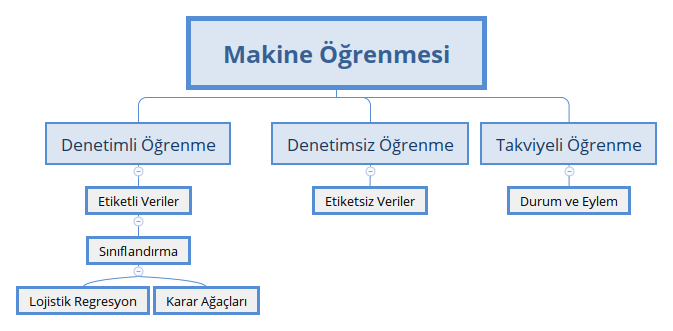
\includegraphics[width=1\linewidth]{figure/makine-ogrenmesi} 

}

\caption{Makine Öğrenmesi}\label{fig:unnamed-chunk-1}
\end{figure}
\hypertarget{denetimli-uxf6ux11frenme}{%
\section{Denetimli Öğrenme}\label{denetimli-uxf6ux11frenme}}

Eğitim verisinde bulunan girdileri ve bunlara ait etiketlenmiş çıktı değerlerini kullanarak model üreten (fonksiyon) ve test kümesi üzerinden bu modeli sınayan öğrenme yöntemidir (Onan, 2015). Örneğin; bir görüntü tanıma çalışması yapıldığını varsayılsın. Hangi görüntünün hangi cisme ait olduğu etiketlenmiş bir veri seti olsun. Bu veri setini ve uygun algoritmayı kullanarak gerçekleştirilen öğrenme türüne \textbf{Denetimli Öğrenme} denilmektedir. Denetimli öğrenme yöntemlerini \textbf{Regresyon} ve \textbf{Sınıflandırma} olarak 2 grupta incelemek mümkündür.

\hypertarget{regresyon}{%
\subsection{Regresyon}\label{regresyon}}

İstatistik biliminin temel ilgi alanlarından olan regresyon, bağımlı bir değişkenin davranışının, bağımsız bir veya daha fazla değişken üzerinden modellenmesidir (Özift, 2014 s, 215). Bağımsız değişkenlere, bağımlı değişkeni etkiledikleri derecede bir katsayı atanır. Hipotez, nicel bağımlı bir değişken tahmin etmeye yöneliktir. Regresyon yöntemleri doğrusal ve doğrusal olmayan regresyon modelleri üzerinden incelenmektedir.

\hypertarget{doux11frusal-regresyon}{%
\subsubsection{Doğrusal Regresyon}\label{doux11frusal-regresyon}}

Regresyon analizinde temel amaç bağımlı değişkeni tahmin edecek en iyi modelin tahmin edilmesidir. Bir diğer ifadeyle bağımlı değişkendeki varyasyonu en iyi açıklayan denklemin oluşturulmasıdır. Regresyon modelindeki bağımsız değişken birinci dereceden ise bu model doğrusal model olarak ifade edilir.

Basit doğrusal regresyon modelinde bir bağımlı (\(\mathrm{Y}\)) ve bir bağımsız değişken (\emph{\(\mathrm{X}\)}) vardır. Çoklu doğrusal regresyon modelinde ise bir bağımlı (\(\mathrm{Y}\)) ve birden fazla bağımsız değişken (\(\mathrm{X_i}\)) vardır.

(X\textsubscript{i} Y\textsubscript{i}) gözlemlerine ait basit doğrusal regresyon modeli aşağıdaki gibidir:

\[
{Y_i}=\alpha+\beta {X_i}+\varepsilon_{i} \quad {i=1,2,\ldots,n}
\]

Burada;
\({X}:\) Bağimsız değişken

\({Y}:\) Bağımlı değişken

\(\alpha:\) Regresyon doğrusunun \({Y}\) eksenini kestiği değer

\(\beta:\) Regresyon doğrusunun eğimidir.

\(\varepsilon:\) hata değerleridir.

\({\varepsilon}\)'nun ortalamasının sıfır, varyansının olduğu ve normal dağılış gösterdiği varsayılır. Bu bir hata değerinin başka bir hata değerinden etkilenmediği anlamına gelir. Yani hata terimleri arasında otokorelasyon yoktur. \(\varepsilon\) değerleri kesin olarak bilinmeyen, pozitif veya negatif değerler alabilen rassal bir değişkendir (Anderson et al.~1981; Gujarati 2005 s,132). Hata terimi Y bağımlı değişkenini etkileyen diğer değişkenlerin modele dahil edilmemesi, modelin yanlış seçilmesi, bilgi kaynağının homojen olmaması ve ölçme yanlışlıklarından dolayı ortaya çıkmaktadır (Kılıçbay 1980; Johnson and Wichern 1998; Gujarati 2005 s,141).

\hypertarget{lojistik-regresyon}{%
\subsubsection{Lojistik Regresyon}\label{lojistik-regresyon}}

Günümüzde biyoloji, tıp, tarım ve ekonomi, gibi alanlarda kolay kullanımı ve yorumlanması nedeniyle lojistik regresyon yaygın olarak kullanılan ve tercih edilen bir yöntem haline gelmiştir.

Doğrusal regresyon modelinden farkı ise, lojistik regresyon analizinde bağımlı değişkenin iki ya da çok sınıflı olmasıdır. Lojistik regresyon ve doğrusal regresyon analizi arasındaki bu farklılık hem parametrik model seçimine hem de varsayımlara yansımaktadır {[}Hosmer, D. W., Lemeshow, S., 1989, 5-50 s,102{]}. Lojistik regresyon, normallik varsayımının bozulması nedeniyle doğrusal regresyon analizine alternatif olmaktadır. Doğrusal regresyon analizinde bağımlı değişkenin değeri, lojistik regresyon analizinde ise bağımlı değişkenin alabileceği değerlerden birinin gerçekleşme olasılığı tahmin edilmektedir. Temel olarak lojistik regresyonda bağımsız değişkenler ile iki ya da çok sınıflı kategorik bağımlı değişken arasındaki ilişkinin tanımlanması için matematiksel modelleme yapmak amaçlanmaktadır {[}Kleinbaum,G., D., 1994 s,76{]}.

Lojistik regresyonun modelleme aşamasında kullanılacak olan lojistik modeli elde etmek için yapılan adımlara aşağıda değinilmiştir.
\[
{y_i}=\sum_{k=0}^{p} \beta_{k} {X_{ik}}+\varepsilon{_i}
\]

şeklinde ifade edilen modelde bağimsiz değiskenler üzerinde bir kısit yoktur. Ayni zamanda \({y_i}\) bağimli değisken değeri de \(-\infty\) ile \(+\infty\) arasinda tüm değerleri alabilmektedir. Bağımlı değiskenin 0 ve 1 gibi değerler aldığı durumda bu kural bozulmakta ve \(P\left({y_i}=1\right)\) \(i\). gözlemin 1 değerini alma olasılığı olmak üzere, beklenen değer:

\[
E\left({y_i}\right)=1 \times P\left({y_i}=1\right)+0 \times P\left({y_i}=0\right)=P\left({y_i}=1\right) \text { olmaktadır. }
\]

Bu sonuç regresyon denklemi olarak yazılacak olursa:

\[
E\left({y_i}\right)=P\left({y_i}=1\right)=\sum_{k=0}^{p} \beta_{k^{x} i k}\quad, {i=1,} \ldots {, n}
\]

ifadesi elde edilmektedir. Sol tarafı. \(0-1\) arasinda olasılık değerleri alan bu denkleme ``Doğrusal olasılık modeli'' adı verilmektedir {[}Tatlıdil, H., 1996 s, 120{]}
Doğrusal olasılık modelinde bağımlı değisken değeri olarak ifade edilen olasılık değerinin çesitli dönüşümlerle - \(-\infty,+\infty\) arasinda tanimlı hale getirilmesi amaciyla yapılacak dönüşümlerden birisi lojit dönüşüm olup. lojit dönüşümde, ilk olarak;

\[
E\left({y_i}\right)=P\left({y_i}=1\right)=\sum_{k=0}^{p} \beta_{k^{x} i k}\quad, {i=1, \ldots, n}
\]
modelinde olasilik değerleri üzerinde \(\frac{P}{1-P} \quad\) dönüsümü yapılarak bağımlı değiskenin sinirları 0,1 yapilmakta, daha sonra ise bu oran değerinin logaritması alınarak bağımlı değişkenin sinirları -\(\infty\), + \(\infty\) yapılmaktadir. Bu dönüşümlerden sonra elde edilen yeni fonksiyon:

\[
g(x)=\ln \left[\frac{\pi(x)}{1-\pi(x)}\right]=\beta_{0}+\beta_{1}X
\]

olarak yazılabilir. Bu modele de ``Lojistik model'' ya da kısaca ``Lojit'' denmektedir. Transformasyon değiskeni \(g(x),\) modeldeki parametreler ile doğrusaldir, süreklidir ve - \(\infty\) ile \(+\infty\) aralığında değisen değerler alir. \(\pi(x)\) arttikça \(g(x)\) 'te artar ve eğer \(\pi(x)<0,5\) ise \(g(x)\) negatif, \(\pi(x)>0,5\) ise \(g(x)\) pozitif değerler alır (Hosmer ve Lemeshov, 1989: 5,307).

\[
{P_i}=\frac{\exp \left(\sum_{k=0}^{p} \beta_{k^{x} i k}\right)}{1+\exp \left(\sum_{k=0}^{p} \beta_{k^{x} i k}\right)}
\]

biçiminde tanimlanmaktadır {[}Collet, D., 2003{]}.

Lojistik analizinde yapılması gereken önemli noktalardan biri kurulan model katsayısinin yorumlanmasidir. Bağımsız bir \({k_x}\) değişkeninin katsayısı \(\beta_{x}, {k_x}\) 'da meydana gelen bir birim değişikliğin y bağımlı değiskeni üzerinde yarattığı değisimin. miktarını ve yönünü vermektedir. Bunun isin öncelikle bağimlı ve bağimsiz değiskenler arasindaki fonksiyonel iliskinin bulunmasi gereklidir. Bir modeldeki bağimsiz değiskenler ile bağımlı değişken arasındaki lineer ilişkiyi veren fonksiyona ``link fonksiyonu'' adı verilmektedir. Bağımlı değiskenin tanimı gereği parametrelerinde doğrusal olan doğrusal regresyon modelinde link fonksiyonu birim fonksiyon (matris) iken; lojistik regresyonda söz konusu fonksiyon logit dönüçümdür. Bu dönüşüm de,

\[
{g(x)}=\ln \left\{\frac{P(x)}{[1-P(x)]}\right\}=\beta_{0}+\beta_{1} {x}
\]

Bu denkleme göre lojistik regresyon modelinde \(\beta_{1}\) katsayısı, \({x}\) bağimsiz değişkeninin bir birim değişiminin lojitte sağlayacağı değişim olup \(\beta_{1}=\) \({g(x+1)-g(x)}\) olarak ifade edimektedir. Yani lojistik regresyon modelinde katsayının yorumu, iki lojit arasındaki farka anlam kazandırılması esasına dayanmaktadır.Buda odds ratio ile ifade edilir.

\hypertarget{odds-oranux131}{%
\paragraph{Odds Oranı}\label{odds-oranux131}}

Odds, başarı ya da görülme olasılığının ``p'', başarısızlık ya da görülmeme olasılığına ``1-p'' oranıdır. Odds ratio iki odds'un birbirine oranıdır. İki değişken arasındaki ilişkinin özet bir ölçüsüdür.

\[
\frac{p /(1-p)}{q /(1-q)}=\frac{p(1-q)}{q(1-p)}
\]

\hypertarget{regresyon-performansux131nux131-uxf6luxe7me-yuxf6ntemleri}{%
\subsubsection{Regresyon Performansını Ölçme Yöntemleri}\label{regresyon-performansux131nux131-uxf6luxe7me-yuxf6ntemleri}}

Kök Ortalama Kare Hatası (Root Mean Square Error - RMSE), modelin çıktısının rakam olduğu durumlarda, modelin tahmin kabiliyetini ölçmek için kullanılan yaygın bir yöntemdir (Chai ve Draxler, 2014). Ortalama Kare Hatası (Mean Square Error - MSE), artıkların karelerinin toplamlarının örnek sayısına bölünmesi ile elde edilir. Burada artıklar, gözlem değerleri ile tahmin değerlerinin farkından oluşur. MSE ölçütüne ait formül şu şekildedir: (\({e_t}\)); değişkeni artıkları temsil etmektedir. RMSE ise MSE değerinin karekökünün alınması ile elde edilir) (Yücalar vd., 2016).

\[
{MSE}=\frac{1}{n} \sum_{t=1}^{n} {e_t}^{2}
\]

Yaygın kullanılan diğer bir ölçüt ise \(R^2\)'dir. \(R^2\), bağımlı değişkenin/değişkenlerin, bağımsız değişkeni, kullanılan model ile ne derece açıkladığını göstermektedir. \(R^2\) değeri 0 ile 1 arasında değerler almaktadır. Bu ölçüt 1'e ne kadar yakın ise modelin değişiminin o derece iyi açıklandığı söylenmektedir.

Yanlılık-Varyans ikilemi: MSE ölçütünün farklı bir şekilde ele alınması olarak düşünülebilmektedir. MSE ölçütü hesaplandığında veri setindeki verilerin birbirinden bağımsız olduğunu, artıkların ortalamasının sıfır, varyansının sabit ve \(\sigma^{2}\) olduğunu varsayılsın. Bu durum şu şekilde bir denklem ile ifade edilir.

\[
\mathrm{E}[\mathrm{MSE}]=\sigma^{2}+(\text { Model yanlılığı})^{2}+\text { model varyansı }
\]

Burada; \textbf{E} beklenen değeri temsil ederken, \(\sigma^{2}\) azaltılamayan gürültü değerini temsil etmektedir. İkinci terim model yanlılık değerinin karesi olup, tahmin edilen değerler ile olması gereken değerler arasındaki yakınlığı temsil etmektedir.
Varyansı düşük olan algoritmalar, karmaşıklığı daha az ve daha sabit alt yapıya sahip algoritmalar iken, yanlılığı düşük olan algoritmalar daha karmaşık ve daha esnek yapıya sahip algoritmalardır (Zhang vd., 2006). Karmaşıklığı çok düşük olan algoritmalar veriye tam uymaz ve veriden yeterince öğrenemezler. Oldukça karmaşık olan algoritmalar ise veriye aşırı uygunluk/uyum (overfitting) gösterirler, yani veriden öğrenmek yerine ezberleme yoluna giderler (Cao ve Tay, 2003 s,210).

İyi bir tahmin modelinde, toplam hatayı en küçükleyecek şekilde yanlılık-varyans dengesi kurulmalıdır. Bunu başarabilmek için izlenebilecek bazı yöntemler şu şekildedir:
\begin{itemize}
\tightlist
\item
  Veriyi eğitim ve test kümesi olarak ayırmak
\item
  Uygun olan algoritmaları denemek
\item
  Model parametrelerini uydurmak
\item
  Etkili parametre ayarlamaları yapmak
\item
  Uygun performans ölçütleri kullanmak
\item
  Sistematik çapraz doğrulama kullanmak
\end{itemize}
\hypertarget{sux131nux131flandux131rma}{%
\subsection{Sınıflandırma}\label{sux131nux131flandux131rma}}

Sınıflandırma, verileri benzerliklerine ve farklılıklarına uygun şekilde birbirlerinden ayırmak/gruplamak için kullanılan bir yöntemdir (Sayad, 2008). Sınıflandırma yöntemleri, veri setinin iki veya çok boyutlu düzlem üzerindeki dağılımına uygun şekilde, birbirine benzer özellikler taşıyan örneklerin her birinin kendi içinde gruplanmasını sağlamak amacıyla, en uygun fonksiyonu belirlemek için kullanılır.

Problemdeki her girdi vektörünü, sonlu sayıdaki bir ayrık kategoriye atamayı amaçlayan durumlar, \textbf{sınıflandırma} (classification) problemi olarak ele alınmaktadır (Bishop, 2007 s,165).

Sınıflandırma problemlerinde çıktı uzayındaki her bir eleman birer \textbf{sınıf} (class), sınıflandırma problemini çözen algoritmaya da \textbf{sınıflandırıcı} (classifier) adı verilmektedir (Camastra ve Vinciarelli, 2008 s,147).

Sınıflandırma, her verinin hangi sınıfa ait olduğu bilindiği bir veri setinin eğitilerek, yeni gelecek bir test verisinin hangi sınıfa ait olduğunun tahmin edilmesi üzerine çalışır.

Makine öğrenmesinde sınıflandırma için kullanılan Naive Bayes Sınıflandırıcı, k-En Yakın Komşu Algoritması, Karar Ağaçları, Yapay Sinir Ağları, Destek Vektör Makineleri gibi çok sayıda algoritma mevcuttur. Bir sınıflandırıcı, bir başka ifade ile bir sınıflandırma modeli (classification model), örneklerden tahmin edilen sınıflara doğru bir haritalamadır (Fawcett, 2006 s,176).

Bu çalışmada karar ağacı algoritmalarından CART algoritması uygulanmıştır.

\hypertarget{cart-algoritmasux131}{%
\subsubsection{CART Algoritması}\label{cart-algoritmasux131}}

CART algoritması, ağaç yapısına dayalı olarak sınıflandırma ve regresyon modellerinin türetilmesi için yaygın olarak kullanılan bir istatistiksel prosedürdür. CART ağaç modeli, tek değişkenli ikili kararların bir hiyerarşisini içerir. CART verileri iki alt kümeye ayırdığı için her bir alt küme içindeki durumlar, bir önceki alt kümeden daha homojen olacaktır. Bu ardışık süreç, homojenlik kriterine ulaşılıncaya veya diğer bazı durma kriterleri sağlanıncaya kadar kendini tekrar eder. Aynı kestirim değişkeni ağaçta farklı düzeylerde pek çok kez kullanılabilir. Ağacın yapısı önceden belirlenmemekte, verilerden türetilmektedir (Answer Tree 3.0 User's Guide, 2001 s,189).

CART, kök düğümünde, verilerin iki gruba bölünmesi için en iyi değişkenin seçilmesini sağlar ve farklı bölümlendirme (splitting) kriterleri kullanır. Bu bölümlendirme kriterlerinin tümü, her bir alt kümedeki sınıf etiketlerini mümkün olduğunca homojen olacak biçimde bölümlendirir (Classification and Regression Trees: An Introduction, 2003: s,12). Bölümlendirme prosedürü çocuk düğümlere (child node) veya alt düğümlerin her birine ardışık olarak uygulanır (Hand, Manila ve Smyth, 2001 s,147).

CART ağaçları, kesin bir heterojenlik (impurity) ölçüsüne bağlı olarak düğümlere ayrılmış iki değerli (binary) ağaçlardır ve bu nedenle de sonuçta homojen dallar oluşmaktadır (Ahola ve Rinta-Runsala, 2001 s,17). Ağacın hedefi benzer veya aynı çıktı değerlerine sahip olma eğiliminde olan alt gruplar yaratmaktır. CART modelleri için bölünmelerin bulunmasında kullanılan dört farklı heterojenlik ölçüsü mevcuttur. Kategorik hedef degişkenler için Gini. Twoing veya (sıralayıcı hedef değişkenleri için) sıralı Twoing. sürekli hedef değişkenler için ise en küçük kareli sapma (LSD) kullanılabilir.

\textbf{Gini indeksi} aşağıdaki şekilde yazılabilir:
\[
g(t)=1-\sum_{j} p^{2}(j / t)
\]
Her hangi bir düğümde durumlar kategoriler arasında eşit biçimde dağıldığında, Gini indeksi \(1-\frac{1}{k}\) maksimum değerini alır. Bir düğümdeki durumlar aynı Bir düğümdeki durumlar aynı kategoriye ait olduğunda ise Gini indeksi 0'a eşit olacaktır (Apte ve Weiss,1997 s,41).

\textbf{Twoing indeksi}, hedef değişken kategorilerinin iki süper sınıfa bölümlendirilmesine dayalıdır ve ardından bu iki süper sınıfa dayalı olarak kestirim değişkenindeki en iyi bölünmeyi bulur. \(t\) düğümünde \(s\) bölünmesi için Twoing kriter fonksiyonu şu şekilde tanımlanabilir (Answer Tree 3.0 User's Guide, 2001 s,194):

\[
\Phi_{(s, t)}=p_{L} p_{R}\left\lfloor\left|\sum_{j} p\left(\frac{j}{t_{L}}-p\left(\frac{j}{t_{R}}\right)\right)\right|\right\rfloor
\]
Fonksiyonda yer alan \({t_{L}}\) ve \({t_{R}}\), s bölünmesi tarafından yaratılan düğümleri göstermektedir. s bölünmesi, bu kriteri maksimize eden bölünme olarak belirlenir. İki süper sınıf olan C1 ve C2 aşağıdaki biçimde tanımlanabilir:

\[
\begin{array}{c}C_{1}=\left\{J: p\left(\frac{j}{t_{L}}\right) \geq p\left(\frac{j}{t_{R}}\right)\right\} \\C_{2}=C-C_{1}\end{array}
\]
Burada \(C\), hedef değişkenin kategori kümesidir.

\textbf{Sıralı Twoing indeksi}, sıralayıcı hedef değişkenleri için Twoing indeksinin değiştirilmiş şeklidir. Sıralı Twoing kriterindeki farklılık yalnızcabitişik kategorilerin süper sınıflar ile birleştirilmesidir. Örneğin bir değişkenin 4 kategorisi olsun. Twoing kriteri i ve 4'ü bir süper sınıf ve 2 ve 3' ü de diğer bir süper sınıf olarak belirlemiş olsun. Bununla beraber kategoriler sıralı olduğundan 1 ve 4 kategorileri birleştirilemez çünkü bunlar bitişik kategoriler değillerdir. Sıralı Twoing indeksi bu durumu göz önüne aldığından i ve 4 gibi kategoriler bitişik olmadığından birleştirilemez.

\textbf{En küçük kareli sapma (LSD)} heterojenlik ölçüsü sürekli hedef değişkenleri için kullanılmaktadır. LSD ölçüsü R(t), t düğümü için basit (ağırlıklandırılmış) düğüm içi varyansıdır ve düğüm için risk tahminine eşittir. R(t)' nin formülü aşağıdaki şekildedir (Answer Tree 3.0 User's Guide,2001 s,195):
\[
R(t)=\frac{1}{N_{w}(t)} \sum w_{n} f_{n}\left(y_{1}-y(t)\right)^{2}
\]
\(N_w(t)\), \(t\) düğümündeki ağırlıklandırılımış durum sayısı, \(w_n\)'nin durumu için mevcut ise ağırlıklandırılımış değişken değeri, \(f_n\) mevcut ise frekans değişkeninin değerini, \(y_1\) hedef değişkenin değerini ve \(y(t)\) ise \(t\) düğümü için ağırlıklı ortalamayı göstermektedir.

Sonuçta elde edilen ağacın büyüklüğü, karmaşık budama sürecinin bir sonucudur. Çok büyük bir ağaç, uyumun üzerinde (overfitting) ve çok küçük ağaç, yetersiz tahmin gücüne sahip olacaktır. Ağaç yapısının hiyerarşik formu, CART gibi algoritmaları ağaç yapısına dayanmayan diğer sınıflandırma algoritmalarından açık bir şekilde ayırır.

\hypertarget{sux131nux131flandux131rma-performansux131nux131-uxf6luxe7me-yuxf6ntemleri}{%
\subsubsection{Sınıflandırma Performansını Ölçme Yöntemleri}\label{sux131nux131flandux131rma-performansux131nux131-uxf6luxe7me-yuxf6ntemleri}}

Regresyon modellemesinde sıkça kullanılan RMSE veya R2 ölçütleri sınıflandırma yöntemlerinin performansını ölçmek için uygun değildir. Bu tarz problemler için kullanılabilecek ölçütlerden bazıları şu şekildedir; Log-Kaybı (Log-Loss), Karmaşıklık Matrisi (Doğruluk), F1 skoru ve Eğri Altında Kalan Alan (Area Under Curve - AUC).

\hypertarget{log-kaybux131}{%
\paragraph{Log-Kaybı}\label{log-kaybux131}}

Logaritmik kayıp oldukça önemli bir performans ölçütüdür. Tahmin değerinin 0 ile 1 arasında bir olasılık değeri olduğu durumlarda sınıflandırma modelinin performansını ölçer. Mükemmel modelin Log-Kaybı değeri sıfırdır. Makine öğrenmesi modelimizin hedefi bu değeri 0'a yaklaştırmak olmalıdır. Örneğin, doğru etiket değeri 1 olan bir örnek için yaptığımız tahminin 0.023 gibi bir değer çıkması, yüksek Log-Kaybı olduğu ve kötü bir model kurulduğu anlamına gelmektedir.

\hypertarget{karmaux15fux131klux131k-hata-matrisi}{%
\paragraph{Karmaşıklık (Hata) Matrisi}\label{karmaux15fux131klux131k-hata-matrisi}}

İki veya çok sınıflı sınıflandırma probleminde, modelin doğruluğunu ölçmek için yaygın şekilde kullanılan ve anlaşılması basit bir matristir. Bu matrisi bir örnek üzerinden açıklamak adına hedef değişkenimiz için aşağıdaki iki etiketi kullandığımızı varsayalım:
\begin{itemize}
\tightlist
\item
  ``0'': Kişide test edilen hastalık bulunmamaktadır.
\item
  ``1'': Kişide test edilen hastalık bulunmaktadır.
\end{itemize}
Bu etiketlerle sınıflandırma yapıldığında oluşacak karmaşıklık matrisi Şekil 1.6'da gösterilmiştir. Matriste yer alan bilgiler kısaca aşağıdaki gibidir:

*\textbf{Doğru Pozitif (DP):} Verinin gerçek değerinin pozitif (1) ve tahmin edilen değerin de pozitif (1) olduğu durum.

*\textbf{Doğru Negatif (DN):} Verinin gerçek değerinin negatif (0) ve tahmin edilen değerin de negatif (0) olduğu durum.

*\textbf{Yanlış Pozitif (YP):} Verinin gerçek değerinin negatif (0) fakat tahmin edilen değerin pozitif (1) olduğu durum.

*\textbf{Yanlış Negatif (YN):} Verinin gerçek değerinin pozitif (1) fakat tahmin edilen değerin negatif (0) olduğu durum.
\begin{longtable}[]{@{}rrcc@{}}
\caption{\label{tab:inher} Karmaşıklık Matrisi}\tabularnewline
\toprule
& & Tahmin Edilen &\tabularnewline
\midrule
\endfirsthead
\toprule
& & Tahmin Edilen &\tabularnewline
\midrule
\endhead
& & Pozitif & Negatif\tabularnewline
Gerçek & Pozitif & DP & YN\tabularnewline
Durum & Negatif & YP & DN\tabularnewline
\bottomrule
\end{longtable}
\hypertarget{doux11fruluk-accuracy}{%
\subparagraph{Doğruluk (Accuracy)}\label{doux11fruluk-accuracy}}

Sınıflandırma problemlerinde doğru tahminlerin bütün tahminlere oranıdır ve hesaplama formülü aşağıdaki gibidir.
\[
\text { Doğruluk }=\frac{D P+D N}{D P+D N+Y P+Y N}
\]
Hedef değişken sınıflarının veri kümesinde dengeli dağıldığı durumlarda Doğruluk ölçütünü kullanmak mantıklıdır. Fakat birçok gerçek hayat probleminde, bu dengeyi yakalamak zordur. Bu dengenin olmadığı ve bir sınıf değerinin çoğunlukta olduğu durumlarda ACC ölçütünün kullanılması önerilmez.

\hypertarget{kesinlik-precision}{%
\subparagraph{Kesinlik (Precision)}\label{kesinlik-precision}}

Kesinlik ölçütü, pozitif tahminde bulunduğumuz verilerin gerçekte hangi oranda pozitif olduğu sorusuna cevap verir ve hesaplama formülü aşağıdaki gibidir.
\[
\text {Kesinlik}=\frac{D P}{D P+Y P}
\]

\hypertarget{hassaslux131k-sensitivity}{%
\subparagraph{Hassaslık (Sensitivity)}\label{hassaslux131k-sensitivity}}

Aynı zamanda `Doğru Pozitif Oranı (DPO)' olarak da adlandırılan bu ölçüt, gerçekte pozitif olanların ne kadarının doğru tahmin edildiğini ölçer ve hesaplama formülü aşağıdaki gibidir.
\[
\text {Hassaslik}=\frac{D P}{D P+Y N}
\]
Kesinlik ölçütü, sınıflandırıcı performansını yanlış pozitifler ile açıklarken, yakalama ölçütü bu performansı yanlış negatifler ile açıklar. Problem tipimize ve hipotezimize bağlı olarak, hangi ölçütü iyileştirmeye çalışacağımızı belirlemeliyiz.

\hypertarget{belirlilik-specifity}{%
\subparagraph{Belirlilik (Specifity)}\label{belirlilik-specifity}}

Aynı zamanda `Doğru Negatif Oranı' olarak da adlandırılan bu ölçüt gerçekte negatif olanların ne kadarının doğru tahmin edildiğini ölçer ve hesaplama formülü aşağıdaki gibidir.

\[
\text {Belirlilik}=\frac{D N}{D N+Y P}
\]

\hypertarget{f1-skoru}{%
\paragraph{F1 Skoru}\label{f1-skoru}}

Her seferinde kesinlik ve yakalama ölçütleri ile ayrı ayrı uğraşmak yerine ikisini birlikte temsil eden bir sınıflandırma performans ölçütü kullanmak mümkündür. Kesinlik ve yakalama ölçütlerinin ağırlıklı ortalamaları ile hesaplanan F1 Skorunun, doğruluk ölçütünden (ACC) daha kullanışlı olduğunu söylemek mümkündür. Hesaplama formülü aşağıdaki gibidir.
\[
\text {F1 Skoru} =\frac{2 * \text { Kesinlik} * \text { Hassaslik }}{\text { Kesinlik }+\text { Hassaslik }}
\]

\hypertarget{sux131nama-ve-geuxe7erleme}{%
\subsection{Sınama ve Geçerleme}\label{sux131nama-ve-geuxe7erleme}}

Denetimli öğrenme uygulamalarında, kullanılan algoritmanın başarısının sınanması için elimizdeki veri kümesinin; eğitim ve test kümesi olarak ayrılması gerekmektedir. Ayırma işlemi çeşitli şekillerde yapılabilir.

\hypertarget{sabit-ayux131rma}{%
\subsubsection{Sabit Ayırma}\label{sabit-ayux131rma}}

Klasik veri ayırma yöntemi olup, veri kümesi \%80 eğitim ve \%20 test olacak şekilde ayrılır (\%66 -- \%34 gibi değerler de kullanılabilir). En büyük dezavantajı, verinin dağılımına göre bazı yanlılık durumlarının ve hataların oluşabilmesidir.

\hypertarget{k-katlamalux131-uxe7apraz-doux11frulama}{%
\subsubsection{K-Katlamalı Çapraz Doğrulama}\label{k-katlamalux131-uxe7apraz-doux11frulama}}

Bu yöntemde veri kümesi k sayısı kadar eşit parçaya bölünür ve her parçanın hem eğitim hem de test için kullanılması sağlanır. Bu sayede test kümesi seçimi yaparken oluşan yanlılık ortadan kaldırılmış olur. Aşağıdaki örnekte, k sayısının 5 seçildiğini düşünelim. Veri kümesi 5 eşit parçaya bölünür ve seçilen algoritma, eğitim ve test aşamalarını bu 5 parçayı da kullanarak gerçekleştirir.
\begin{itemize}
\tightlist
\item
  Model 1: (Parça 1 + Parça 2 + Parça 3 + Parça 4) eğitim kümesi, Parça 5 test kümesi
\item
  Model 2: (Parça 1 + Parça 2 + Parça 3 + Parça 5) eğitim kümesi, Parça 4 test kümesi
\item
  Model 3: (Parça 1 + Parça 2 + Parça 4 + Parça 5) eğitim kümesi, Parça 3 test kümesi
\item
  Model 4: (Parça 1 + Parça 3 + Parça 4 + Parça 5) eğitim kümesi, Parça 2 test kümesi
\item
  Model 5: (Parça 2 + Parça 3 + Parça 4 + Parça 5) eğitim kümesi, Parça 1 test kümesi
\end{itemize}
\begin{figure}

{\centering 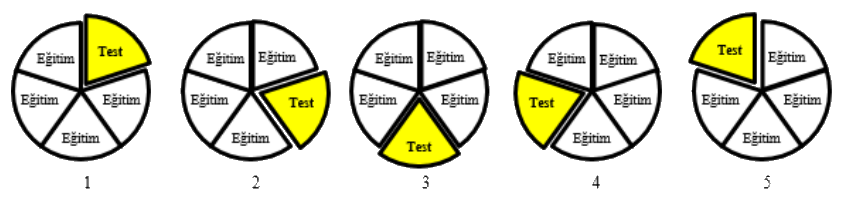
\includegraphics[width=1\linewidth]{figure/kk} 

}

\caption{K-Katlamalı Çapraz Doğrulama}\label{fig:unnamed-chunk-2}
\end{figure}
\hypertarget{denetimsiz-uxf6ux11frenme}{%
\section{Denetimsiz Öğrenme}\label{denetimsiz-uxf6ux11frenme}}

Veri kümesindeki örneklerin herhangi bir etiketle (sınıfla) ayrıştırılmadığı ve etiket sayısının bilinmediği durumda kullanılan öğrenme yöntemidir (Yıldırım ve Birant, 2018). Literatürde en çok kullanılan denetimsiz öğrenme yöntemi, birbirine benzeyen örneklerin bir araya getirilmesini (gruplanmasını/kümelenmesini) amaçlayan Kümelemedir. Örneğin, bir alışveriş sitesini ele alalım. Siteyi kullanan müşterilerin farklı özelliklerini ve geçmişte yaptıkları, site içi gezinme, sepete atma, alışveriş yapma vb. bilgileri barındıran bir veri kümesinde, benzer davranışları gerçekleştiren müşterileri gruplamak mümkündür.

Kümeleme yöntemlerinin çoğu, veri örnekleri arasındaki uzaklık/yakınlık bilgisini kullanarak benzerlik bulma ve gruplama işlemini gerçekleştirmektedir. Verilerin benzerliğinin bulunmasında, basit bir uzaklık ölçütü (Öklid, Manhattan, Minkowski) kullanılabilir. Bunun dışında, yoğunluk ve komşuluk gibi özel hesaplamalar da benzerlik bulma için kullanılabilir.

Kümeleme işleminde kullanılan 5 farklı veri gruplama yaklaşımı bulunmaktadır.
\begin{enumerate}
\def\labelenumi{\arabic{enumi}.}
\tightlist
\item
  Bölümleme Tabanlı (Partitioning) Yöntemler (K-Ortalamalar, K-Medoid, PAM, CLARA)
\item
  Hiyerarşik Yöntemler (AGNES, DIANA)
\item
  Yoğunluk Tabanlı Yöntemler (DBSCAN, OPTICS)
\item
  Model Tabanlı Yöntemler (EM)
\item
  Izgara Tabanlı Yöntemler (CLIQUE)
\end{enumerate}
\hypertarget{sonuuxe7larux131-iux307yileux15ftirme}{%
\subsection{Sonuçları İyileştirme}\label{sonuuxe7larux131-iux307yileux15ftirme}}

Bir veri bilimi çalışması yaparken verimli ve yüksek performanslı bir model oluşturmak kolay değildir. Genellikle en büyük çaba, veri keşfi ve doğru makine öğrenmesi algoritmasını seçmek üzerine olsa da sonuçları iyileştirmek için yapacağımız çalışmalara projenin en başından itibaren başlamalıyız. Aynı zamanda şunu da unutmamak gerekir; bir makine öğrenmesi uygulaması yaparken, kullandığımız algoritma veya algoritmaların performansları bize makul derece iyi görünebilir, fakat elde ettiğimizin en iyi sonuç olup olmadığını tek seferde bilemeyiz. Dolayısıyla, birkaç yöntem kullanarak, elde ettiğimiz sonuçların iyileştirilmesi üzerine çalışmalar yapmamız sağlıklı olacaktır.

\textbf{Algoritma Ayarı (Algorithm Tuning):} Birçok gerçek hayat probleminde kullanılan algoritma, var olan (varsayılan) parametreleri ile en iyi sonucu vermeyebilir. En iyi sonucu elde etmek için belli bir kalıbı kullanmak yerine, çalışılan veri kümesine ve algoritmaya özel algoritma parametre ayarı yapılması önemlidir. Bu aşamada ilk yapılması gereken, algoritmanın parametreleri için birden fazla kombinasyonun denenerek en iyi alınan sonuçları saklamaktır. Daha sonra saklanan parametreler üzerinde küçük değişiklikler yapılarak daha iyi bir sonuç elde etmeye çalışılabilir.

\textbf{Topluluk Yöntemleri (Ensemble Methods):} Topluluk yöntemleri adından da anlaşılabileceği üzere, birden çok sonucu birlikte değerlendirmeyi ifade eder. Problemin yapısına göre tamamını çözmek için bir algoritma kullanmaktansa birçok aşamasında birden fazla algoritma kullanılabilir. Birden çok algoritmanın sonuçlarını birleştirerek alacağımız sonuç, yalnızca bir yöntem izleyerek alacağımız çözümden daha performanslı olacaktır.

\textbf{Veri Miktarını Büyütme:} Birçok deneme yapmamıza rağmen tahminlerimiz yüksek varyansa sahip olabilir. Her senaryoda veri miktarını büyütmek mümkün olmayabilir, bu tarz durumlarda diğer bir seçenek de eğitim veri kümesini büyütmek olabilir. Örnek sayısını yeni verilerle büyüterek algoritmanın daha iyi öğrenmesini sağlayabiliriz.

\hypertarget{Bolum4}{%
\chapter{Uygulama}\label{Bolum4}}

İzmir ili Torbalı ilçesinde plastik masa örtüsü üretimi gerçekleştiren SANEM PLASTİK adlı fabrikadan alınan 2018-2019 yılları arasındaki veriler ile sınıflandırma makine öğrenimi algoritmalarını kullanılarak oluşturulan modellere göre fabrikanın verimliliğini arttırmaktır.

~

Fabrikadan alınan veri ``csv'' formatında olduğu için RStudio üzerinden aşağıdaki kod ile data frame veri yapısında ``veri'' adı ile kaydedilmiştir. Daha sonra veri setindeki değişkenlerin yapıları Tablo 4.1'de verilmiştir.
\begin{Shaded}
\begin{Highlighting}[]
\KeywordTok{library}\NormalTok{(readr)}
\NormalTok{veri \textless{}{-}}\StringTok{ }\KeywordTok{read\_delim}\NormalTok{(}\StringTok{"veri.csv"}\NormalTok{, }\StringTok{","}\NormalTok{, }\DataTypeTok{escape\_double =} \OtherTok{FALSE}\NormalTok{, }
    \DataTypeTok{col\_types =} \KeywordTok{cols}\NormalTok{(}\DataTypeTok{tecrube =} \KeywordTok{col\_factor}\NormalTok{(}\DataTypeTok{levels =} \KeywordTok{c}\NormalTok{(}\StringTok{"0"}\NormalTok{, }
        \StringTok{"1"}\NormalTok{)),}\DataTypeTok{gun =} \KeywordTok{col\_factor}\NormalTok{(}\DataTypeTok{levels =} \KeywordTok{c}\NormalTok{(}\StringTok{"1"}\NormalTok{, }
        \StringTok{"2"}\NormalTok{, }\StringTok{"3"}\NormalTok{, }\StringTok{"4"}\NormalTok{, }\StringTok{"5"}\NormalTok{, }\StringTok{"6"}\NormalTok{)), }\DataTypeTok{hafta =} \KeywordTok{col\_factor}\NormalTok{(}\DataTypeTok{levels =} 
        \KeywordTok{c}\NormalTok{(}\StringTok{"Hafta 01"}\NormalTok{,}\StringTok{"Hafta 02"}\NormalTok{, }\StringTok{"Hafta 03"}\NormalTok{, }\StringTok{"Hafta 04"}\NormalTok{, }\StringTok{"Hafta 05"}\NormalTok{, }
        \StringTok{"Hafta 06"}\NormalTok{, }\StringTok{"Hafta 07"}\NormalTok{, }\StringTok{"Hafta 08"}\NormalTok{, }\StringTok{"Hafta 09"}\NormalTok{, }\StringTok{"Hafta 10"}\NormalTok{,}
        \StringTok{"Hafta 11"}\NormalTok{, }\StringTok{"Hafta 12"}\NormalTok{, }\StringTok{"Hafta 13"}\NormalTok{, }\StringTok{"Hafta 14"}\NormalTok{, }\StringTok{"Hafta 15"}\NormalTok{, }
        \StringTok{"Hafta 16"}\NormalTok{, }\StringTok{"Hafta 17"}\NormalTok{, }\StringTok{"Hafta 18"}\NormalTok{, }\StringTok{"Hafta 19"}\NormalTok{,}\StringTok{"Hafta 20"}\NormalTok{,}
        \StringTok{"Hafta 21"}\NormalTok{, }\StringTok{"Hafta 22"}\NormalTok{, }\StringTok{"Hafta 23"}\NormalTok{, }\StringTok{"Hafta 24"}\NormalTok{, }\StringTok{"Hafta 25"}\NormalTok{, }
        \StringTok{"Hafta 26"}\NormalTok{, }\StringTok{"Hafta 27"}\NormalTok{, }\StringTok{"Hafta 28"}\NormalTok{, }\StringTok{"Hafta 29"}\NormalTok{,}\StringTok{"Hafta 30"}\NormalTok{, }
        \StringTok{"Hafta 31"}\NormalTok{, }\StringTok{"Hafta 32"}\NormalTok{, }\StringTok{"Hafta 33"}\NormalTok{, }\StringTok{"Hafta 34"}\NormalTok{, }\StringTok{"Hafta 35"}\NormalTok{, }
        \StringTok{"Hafta 36"}\NormalTok{, }\StringTok{"Hafta 37"}\NormalTok{, }\StringTok{"Hafta 38"}\NormalTok{, }\StringTok{"Hafta 39"}\NormalTok{,}\StringTok{"Hafta 40"}\NormalTok{, }
        \StringTok{"Hafta 41"}\NormalTok{, }\StringTok{"Hafta 42"}\NormalTok{, }\StringTok{"Hafta 43"}\NormalTok{, }\StringTok{"Hafta 44"}\NormalTok{, }\StringTok{"Hafta 45"}\NormalTok{,}
        \StringTok{"Hafta 46"}\NormalTok{)), }\DataTypeTok{tarih =} \KeywordTok{col\_date}\NormalTok{(}\DataTypeTok{format =} \StringTok{"\%Y{-}\%m{-}\%d"}\NormalTok{)), }
    \DataTypeTok{locale =} \KeywordTok{locale}\NormalTok{(}\DataTypeTok{decimal\_mark =} \StringTok{"."}\NormalTok{), }
    \DataTypeTok{trim\_ws =} \OtherTok{TRUE}\NormalTok{)}
\end{Highlighting}
\end{Shaded}
\begin{longtable}[]{@{}lll@{}}
\caption{\label{tab:inher} Veri Seti Değişkenleri}\tabularnewline
\toprule
Değişkenler & Tür & Kategorik\tabularnewline
\midrule
\endfirsthead
\toprule
Değişkenler & Tür & Kategorik\tabularnewline
\midrule
\endhead
OEE \emph{(Hedef Değişken)} & Sürekli &\tabularnewline
& &\tabularnewline
Hafta & Kategorik & 1'den 46'ya kadar\tabularnewline
& &\tabularnewline
Üretim & Sürekli &\tabularnewline
& &\tabularnewline
Tarih & Tarih & Ay- Gün- Yıl\tabularnewline
& &\tabularnewline
Saat & Sürekli & 1 -- 24\tabularnewline
& &\tabularnewline
Kayıp metre & Sürekli &\tabularnewline
& &\tabularnewline
Gün & Kategorik & 1: Pazartesi\tabularnewline
& & 2: Salı\tabularnewline
& & 3: Çarşamba\tabularnewline
& & 4: Perşembe\tabularnewline
& & 5: Cuma\tabularnewline
& & 6: Cumartesi\tabularnewline
& & 7: Pazar\tabularnewline
& &\tabularnewline
On Yıl Tecrübe & Kategorik & 0: On yıl tecrübe altı\tabularnewline
(Simülasyon) & & 1: On yıl tecrübe ve üstü\tabularnewline
\bottomrule
\end{longtable}
Tablo 4.1'de görüldüğü üzere OEE değişkeni bağımlı değişken iken diğer değişkenler bağımsız olarak ele alınmıştır. OEE, üretim, saat, kayıp metre, değişkenleri sürekli, hafta, gün ve tecrübe değişkenleri kategorik değişkenlerdir. Tüm bu değişkenlerin ilk 6 satırının görüntüsü ve özet istatistikleri aşağıda verilmiştir.
\begin{Shaded}
\begin{Highlighting}[]
\KeywordTok{head}\NormalTok{(veri)}
\end{Highlighting}
\end{Shaded}
\begin{verbatim}
# A tibble: 6 x 8
  tarih      hafta    uretim   OEE  saat kayip_metre gun   tecrube
  <date>     <fct>     <dbl> <dbl> <dbl>       <dbl> <fct> <fct>  
1 2019-01-10 Hafta 02  72810    75   5.5       21600 4     0      
2 2019-01-11 Hafta 02  88195    92   2          7802 5     1      
3 2019-01-12 Hafta 02  84400    85   3.6       13846 6     1      
4 2019-01-14 Hafta 03  11800    36   4.1       16118 1     0      
5 2019-01-15 Hafta 03  85780    89   2.7       10473 2     1      
6 2019-01-16 Hafta 03  89530    94   1.5        5795 3     1      
\end{verbatim}
\begin{Shaded}
\begin{Highlighting}[]
\KeywordTok{summary}\NormalTok{(veri)}
\end{Highlighting}
\end{Shaded}
\begin{verbatim}
     tarih                 hafta         uretim           OEE        
 Min.   :2019-01-10   Hafta 16:  6   Min.   : 4750   Min.   : 29.00  
 1st Qu.:2019-03-28   Hafta 22:  6   1st Qu.:49889   1st Qu.: 82.00  
 Median :2019-06-15   Hafta 27:  6   Median :80145   Median : 89.00  
 Mean   :2019-06-16   Hafta 34:  6   Mean   :68018   Mean   : 85.15  
 3rd Qu.:2019-09-10   Hafta 35:  6   3rd Qu.:86760   3rd Qu.: 93.75  
 Max.   :2019-11-13   Hafta 37:  6   Max.   :94680   Max.   :100.00  
                      (Other) :162                                   
      saat         kayip_metre    gun    tecrube
 Min.   : 0.200   Min.   : 1021   1:27   0: 83  
 1st Qu.: 1.000   1st Qu.: 3806   2:36   1:115  
 Median : 1.950   Median : 6943   3:38          
 Mean   : 2.576   Mean   : 8728   4:38          
 3rd Qu.: 3.000   3rd Qu.:11651   5:34          
 Max.   :23.400   Max.   :36471   6:25          
                                                
\end{verbatim}
Modellerin amacı bağımsız değişkenlerin, OEE puanına nasıl etkileyeceğini araştırmaktır. Model için sürekli değişkenlerimiz, ortalamaya göre bölünüp 0-1 olarak kategorik değişken haline getirilmiştir.
\begin{Shaded}
\begin{Highlighting}[]
\NormalTok{veri}\OperatorTok{$}\NormalTok{uretim[veri}\OperatorTok{$}\NormalTok{uretim}\OperatorTok{\textless{}}\KeywordTok{mean}\NormalTok{(veri}\OperatorTok{$}\NormalTok{uretim)]=}\DecValTok{0}
\NormalTok{veri}\OperatorTok{$}\NormalTok{uretim[}\OperatorTok{!}\NormalTok{(veri}\OperatorTok{$}\NormalTok{uretim}\OperatorTok{\textless{}}\KeywordTok{mean}\NormalTok{(veri}\OperatorTok{$}\NormalTok{uretim))]=}\DecValTok{1}
\NormalTok{veri}\OperatorTok{$}\NormalTok{uretim=}\KeywordTok{as.factor}\NormalTok{(veri}\OperatorTok{$}\NormalTok{uretim)}
\end{Highlighting}
\end{Shaded}
\begin{Shaded}
\begin{Highlighting}[]
\NormalTok{veri}\OperatorTok{$}\NormalTok{kayip\_metre[veri}\OperatorTok{$}\NormalTok{kayip\_metre}\OperatorTok{\textless{}}\KeywordTok{mean}\NormalTok{(veri}\OperatorTok{$}\NormalTok{kayip\_metre)]=}\DecValTok{0}
\NormalTok{veri}\OperatorTok{$}\NormalTok{kayip\_metre[}\OperatorTok{!}\NormalTok{(veri}\OperatorTok{$}\NormalTok{kayip\_metre}\OperatorTok{\textless{}}\KeywordTok{mean}\NormalTok{(veri}\OperatorTok{$}\NormalTok{kayip\_metre))]=}\DecValTok{1}
\NormalTok{veri}\OperatorTok{$}\NormalTok{kayip\_metre=}\KeywordTok{as.factor}\NormalTok{(veri}\OperatorTok{$}\NormalTok{kayip\_metre)}
\end{Highlighting}
\end{Shaded}
\begin{Shaded}
\begin{Highlighting}[]
\NormalTok{veri}\OperatorTok{$}\NormalTok{saat[veri}\OperatorTok{$}\NormalTok{saat}\OperatorTok{\textless{}}\KeywordTok{mean}\NormalTok{(veri}\OperatorTok{$}\NormalTok{saat)]=}\DecValTok{0}
\NormalTok{veri}\OperatorTok{$}\NormalTok{saat[}\OperatorTok{!}\NormalTok{(veri}\OperatorTok{$}\NormalTok{saat}\OperatorTok{\textless{}}\KeywordTok{mean}\NormalTok{(veri}\OperatorTok{$}\NormalTok{saat))]=}\DecValTok{1}
\NormalTok{veri}\OperatorTok{$}\NormalTok{saat=}\KeywordTok{as.factor}\NormalTok{(veri}\OperatorTok{$}\NormalTok{saat)}
\end{Highlighting}
\end{Shaded}
Daha önce belirtildiği üzere hedef değişkenimiz OEE değişkenidir. OEE, ``Overall Equipment Effectiveness'' kısaltmasıdır. Türkçe çevirisi Toplam Ekipman Etkinliği'dir. OEE bütün ekipmanların ne ölçüde kullanıldığına işaret eden bir TPM(Total Productive Maintenance) hesabıdır. Arızalar, ekipman ayarları, duruşlar, çalışma hızındaki azalmalar, ıskartalar ve yeniden işlem gibi kayıplar üzerine düşer. Amacı; şirketlerin eldeki makine ve ekipmanların performanslarının arttırılmasına odaklanmaktır. Gerekli görüldüğü ölçüde başka önemli ölçütlerin eklenebilmesi esnekliğine sahip olmasıyla beraber genel olarak 3 önemli değişkeni bir arada hesap eder:

~

OEE {[}\%{]} = Kullanılabilirlik Oranı x Performans Oranı x Kalite Oranı
\begin{itemize}
\item
  \textbf{Kullanılabilirlik Oranı {[}\%{]}:} Ekipmana ait sebeplerden (arıza, ayarlamadan kaynaklanan duruş süresi vs.) kaynaklanan kullanılabilirlik miktarını gösterir.
\item
  \textbf{Performans Oranı {[}\%{]}:} Çalışma hızlarında tasarımla belirlenmiş hızlara göre düşüşleri ve birkaç saniyelik duruşları hesap eder.
\item
  \textbf{Kalite Oranı {[}\%{]}:} Toplam işlenen parçaların ıskarta ve yeniden işlem kayıplarının yüzdesidir. {[}\url{https://lean.org.tr/oee-nedir/}, Can YÜKSELEN{]}
\end{itemize}
Uygulanabilen en iyi OEE değeri \%85 olarak kabul edilmektedir ve bu seviyedeki şirketler \textbf{``World Class''} üretim yapan şirketler olarak anılırlar. Dünya standartlarında olan şirketler OEE performanslarını yükselterek, kapasite ihtiyaçlarını karşılamaya çalışırlar. Böylece kendilerini ek yatırım, ek alan kullanımı, ek işçilik, fazla stok, fazla enerji kullanımı, kalitesizlik ve finansman maliyetlerinden korurlar. Bu nedenle hedef değişken 85 puan ve üstü ile 85 puan altı olarak ayırdık ve 1-0 değerleri ile kategorik değişken olarak değiştirildi.
\begin{Shaded}
\begin{Highlighting}[]
\NormalTok{veri}\OperatorTok{$}\NormalTok{OEE[veri}\OperatorTok{$}\NormalTok{OEE}\OperatorTok{\textless{}}\DecValTok{85}\NormalTok{]=}\DecValTok{0}
\NormalTok{veri}\OperatorTok{$}\NormalTok{OEE[}\OperatorTok{!}\NormalTok{veri}\OperatorTok{$}\NormalTok{OEE}\OperatorTok{\textless{}}\DecValTok{85}\NormalTok{]=}\DecValTok{1}
\NormalTok{veri}\OperatorTok{$}\NormalTok{OEE=}\KeywordTok{as.factor}\NormalTok{(veri}\OperatorTok{$}\NormalTok{OEE)}
\end{Highlighting}
\end{Shaded}
Yeni durumda özet istatistikler şu şekildedir:
\begin{Shaded}
\begin{Highlighting}[]
\KeywordTok{summary}\NormalTok{(veri[,}\OperatorTok{{-}}\DecValTok{1}\NormalTok{])}
\end{Highlighting}
\end{Shaded}
\begin{verbatim}
      hafta     uretim  OEE     saat    kayip_metre gun    tecrube
 Hafta 16:  6   0: 72   0: 68   0:132   0:124       1:27   0: 83  
 Hafta 22:  6   1:126   1:130   1: 66   1: 74       2:36   1:115  
 Hafta 27:  6                                       3:38          
 Hafta 34:  6                                       4:38          
 Hafta 35:  6                                       5:34          
 Hafta 37:  6                                       6:25          
 (Other) :162                                                     
\end{verbatim}
Daha sonra veri \%80 eğitim ve \%20 test olarak iki parçaya aşağıdaki gibi ayrılmıştır.
\begin{Shaded}
\begin{Highlighting}[]
\KeywordTok{set.seed}\NormalTok{(}\DecValTok{1}\NormalTok{)}
\NormalTok{r=}\KeywordTok{as.logical}\NormalTok{(}\KeywordTok{rbinom}\NormalTok{(}\KeywordTok{length}\NormalTok{(veri}\OperatorTok{$}\NormalTok{OEE),}\DecValTok{1}\NormalTok{,}\DataTypeTok{prob =} \FloatTok{0.8}\NormalTok{))}
\NormalTok{train=veri[r,}\OperatorTok{{-}}\KeywordTok{c}\NormalTok{(}\DecValTok{1}\NormalTok{,}\DecValTok{2}\NormalTok{)]}
\NormalTok{test=veri[}\OperatorTok{!}\NormalTok{r,}\OperatorTok{{-}}\KeywordTok{c}\NormalTok{(}\DecValTok{1}\NormalTok{,}\DecValTok{2}\NormalTok{)]}
\end{Highlighting}
\end{Shaded}
\hypertarget{lojistik-regresyon-modeli-full-model}{%
\subsubsection{Lojistik Regresyon Modeli (Full Model)}\label{lojistik-regresyon-modeli-full-model}}

Veri setindeki tüm değişkenlerle train verisi üzerinde lojistik regresyon modeli kurulmuştur. Lojistik regresyon için yapılan full modelin R çıktısı aşağıda verilmektedir.
\begin{Shaded}
\begin{Highlighting}[]
\NormalTok{full.model =}\StringTok{ }\KeywordTok{glm}\NormalTok{(OEE }\OperatorTok{\textasciitilde{}}\NormalTok{. }\OperatorTok{{-}}\StringTok{ }\NormalTok{tecrube ,}\DataTypeTok{family=}\NormalTok{binomial, }\DataTypeTok{data=}\NormalTok{train)}
\KeywordTok{summary}\NormalTok{(full.model)}
\end{Highlighting}
\end{Shaded}
\begin{verbatim}
Call:
glm(formula = OEE ~ . - tecrube, family = binomial, data = train)

Deviance Residuals: 
    Min       1Q   Median       3Q      Max  
-2.7868  -0.4047   0.2040   0.6068   1.4250  

Coefficients:
             Estimate Std. Error z value Pr(>|z|)    
(Intercept)  -0.14138    0.54440  -0.260  0.79509    
uretim1       3.90538    0.80857   4.830 1.37e-06 ***
saat1        -2.21958    0.86006  -2.581  0.00986 ** 
kayip_metre1 -1.90456    1.00137  -1.902  0.05718 .  
gun2          0.09838    0.73493   0.134  0.89351    
gun3         -0.20531    0.75528  -0.272  0.78575    
gun4         -0.03542    0.73268  -0.048  0.96144    
gun5          1.07417    0.82050   1.309  0.19048    
gun6          1.56849    0.87277   1.797  0.07231 .  
---
Signif. codes:  0 '***' 0.001 '**' 0.01 '*' 0.05 '.' 0.1 ' ' 1

(Dispersion parameter for binomial family taken to be 1)

    Null deviance: 214.49  on 162  degrees of freedom
Residual deviance: 120.85  on 154  degrees of freedom
AIC: 138.85

Number of Fisher Scoring iterations: 6
\end{verbatim}
Çıktıda görüldüğü üzere üretim, saat anlamlı çıkmıştır. Kayıp metre değişkeni 0.05 sınırında olduğundan `.' ile işaretlenmiştir.
Yapılan Korelasyon analizine göre kayıp metre ve saat değişkeni ile ilişkili bulunmuştur (0.48). Bu yüzden kayıp metrenin modele alınmamasına karar verilmiştir.

\hypertarget{lojistik-regresyon-modeli-en-iux307yi-model}{%
\subsubsection{Lojistik Regresyon Modeli (En İyi Model)}\label{lojistik-regresyon-modeli-en-iux307yi-model}}

En iyi modeli oluşturmak için stepwise yöntemi kullanılmıştır. Bu yöntemde modele hem değişken ekleme hem çıkarma işlemlerini uygulaması için direction = ``both'' olarak tanımlanmıştır. En iyi modelin modelin R çıktısı aşağıda verilmektedir.
\begin{Shaded}
\begin{Highlighting}[]
\NormalTok{best.model \textless{}{-}}\StringTok{ }\KeywordTok{stepAIC}\NormalTok{(}\KeywordTok{glm}\NormalTok{(OEE }\OperatorTok{\textasciitilde{}}\NormalTok{. }\OperatorTok{{-}}\StringTok{ }\NormalTok{tecrube }\OperatorTok{{-}}\NormalTok{kayip\_metre ,}\DataTypeTok{family=}\NormalTok{binomial, }\DataTypeTok{data=}\NormalTok{train), }\DataTypeTok{direction =} \StringTok{"both"}\NormalTok{,}\DataTypeTok{trace =} \OtherTok{FALSE}\NormalTok{)}
\KeywordTok{summary}\NormalTok{(best.model)}
\end{Highlighting}
\end{Shaded}
\begin{verbatim}
Call:
glm(formula = OEE ~ uretim + saat, family = binomial, data = train)

Deviance Residuals: 
    Min       1Q   Median       3Q      Max  
-2.5993  -0.2757   0.2635   0.6622   1.2583  

Coefficients:
            Estimate Std. Error z value Pr(>|z|)    
(Intercept)   0.2805     0.3149   0.891    0.373    
uretim1       3.0630     0.6392   4.792 1.65e-06 ***
saat1        -3.5317     0.6397  -5.521 3.38e-08 ***
---
Signif. codes:  0 '***' 0.001 '**' 0.01 '*' 0.05 '.' 0.1 ' ' 1

(Dispersion parameter for binomial family taken to be 1)

    Null deviance: 214.49  on 162  degrees of freedom
Residual deviance: 131.67  on 160  degrees of freedom
AIC: 137.67

Number of Fisher Scoring iterations: 6
\end{verbatim}
Çıktıda görüldüğü üzere en iyi modelde üretim, saat değişkenleri \%95 anlamlılık düzeyinde istatistiksel olarak anlamlı çıkmıştır. Daha sonra OR, CI ve Wald testine bakılmıştır.
\begin{Shaded}
\begin{Highlighting}[]
\KeywordTok{wald.test}\NormalTok{(}\DataTypeTok{b=}\KeywordTok{coef}\NormalTok{(best.model),}\DataTypeTok{Sigma=}\KeywordTok{vcov}\NormalTok{(best.model),}\DataTypeTok{Terms=}\DecValTok{1}\OperatorTok{:}\DecValTok{2}\NormalTok{)}
\end{Highlighting}
\end{Shaded}
\begin{verbatim}
Wald test:
----------

Chi-squared test:
X2 = 31.2, df = 2, P(> X2) = 1.6e-07
\end{verbatim}
Kategorik değişkenlerle kurulan lojistik regresyon en iyi modelindeki Wald değerlerine bakıldığında, tüm p değerleri 0.05'den küçük olduğu için katsayılar \%95 güven seviyesinde istatistiksel olarak anlamlı bulunmuştur.
\begin{Shaded}
\begin{Highlighting}[]
\KeywordTok{exp}\NormalTok{(}\KeywordTok{confint}\NormalTok{(best.model))}
\end{Highlighting}
\end{Shaded}
\begin{verbatim}
Waiting for profiling to be done...
\end{verbatim}
\begin{verbatim}
                  2.5 %      97.5 %
(Intercept) 0.715917230  2.48285748
uretim1     7.032365088 93.58095767
saat1       0.006676091  0.08888818
\end{verbatim}
Ayrıca OR ve güven aralıklarına bakıldığında, OR'a ait güven aralıklarının 1'i içermediği görülmektedir. Bu yüzden OR'ler anlamlıdır ve yorumlanabilir.
\begin{Shaded}
\begin{Highlighting}[]
\KeywordTok{exp}\NormalTok{(}\KeywordTok{coef}\NormalTok{(best.model))}
\end{Highlighting}
\end{Shaded}
\begin{verbatim}
(Intercept)     uretim1       saat1 
 1.32378898 21.39165960  0.02925425 
\end{verbatim}
Üretimi yüksek olanların, üretimi düşük olanlara göre Toplam Ekipman Etkinliğinin (OEE) yüzdesinin yüksek olma şansı yaklaşık olarak 21 katıdır.
Saat değişkeninde ise saati az olanların, yüksek olanlara göre OEE yüzdesinin yüksek olma şansı ise 1/0.29 oranından yaklaşık olarak 3 katı olduğu elde edilmektedir.

Train verisinde oluşturduğumuz model, test verisinde sınıflandırma performansını ölçme yöntemleri ile şu şekilde test edilmiştir.
\begin{Shaded}
\begin{Highlighting}[]
\CommentTok{\#Tahmin Değerleri}
\NormalTok{pred =}\StringTok{ }\KeywordTok{predict}\NormalTok{(best.model, test, }\DataTypeTok{type =} \StringTok{"response"}\NormalTok{)}
\KeywordTok{print}\NormalTok{(}\KeywordTok{round}\NormalTok{(pred,}\DecValTok{2}\NormalTok{))}
\end{Highlighting}
\end{Shaded}
\begin{verbatim}
   1    2    3    4    5    6    7    8    9   10   11   12   13   14   15   16 
0.04 0.97 0.97 0.97 0.97 0.57 0.97 0.97 0.04 0.04 0.45 0.97 0.57 0.97 0.45 0.57 
  17   18   19   20   21   22   23   24   25   26   27   28   29   30   31   32 
0.57 0.57 0.57 0.04 0.57 0.97 0.45 0.97 0.97 0.97 0.97 0.97 0.97 0.97 0.97 0.97 
  33   34   35 
0.97 0.97 0.57 
\end{verbatim}
Tahmin değerleri logistic regresyon modelinde sigmoid fonksiyon gereği 0 ile 1 arasında değerler almaktadır. Bu değerleri kategorik hale getirdiğimiz OEE değişkenindeki 0 ile 1 değerleri gibi tam hale çevirmek için şu kod kullanılmıştır.
\begin{Shaded}
\begin{Highlighting}[]
\NormalTok{pred =}\StringTok{ }\KeywordTok{ifelse}\NormalTok{(pred}\OperatorTok{\textless{}}\FloatTok{0.5}\NormalTok{,}\DecValTok{0}\NormalTok{,}\DecValTok{1}\NormalTok{)}
\KeywordTok{print}\NormalTok{(pred)}
\end{Highlighting}
\end{Shaded}
\begin{verbatim}
 1  2  3  4  5  6  7  8  9 10 11 12 13 14 15 16 17 18 19 20 21 22 23 24 25 26 
 0  1  1  1  1  1  1  1  0  0  0  1  1  1  0  1  1  1  1  0  1  1  0  1  1  1 
27 28 29 30 31 32 33 34 35 
 1  1  1  1  1  1  1  1  1 
\end{verbatim}
\begin{verbatim}
En İyi Model için OEE Karmaşıklık Matrisi 
\end{verbatim}
\begin{verbatim}
          Reference
Prediction  <85  >=85
       <85    5     2
      >=85    3    25
\end{verbatim}
\begin{longtable}[]{@{}lllll@{}}
\toprule
Doğruluk & Kesinlik & Hassaslık & Belirlilik & F1 Skoru\tabularnewline
\midrule
\endhead
0.857 & 0.625 & 0.926 & 0.714 & 0.667\tabularnewline
\bottomrule
\end{longtable}
\hypertarget{cart-algoritmasux131-en-iux307yi-model}{%
\subsubsection{CART Algoritması (En İyi Model)}\label{cart-algoritmasux131-en-iux307yi-model}}
\begin{Shaded}
\begin{Highlighting}[]
\NormalTok{cart=}\KeywordTok{rpart}\NormalTok{(}\DataTypeTok{formula =}\NormalTok{ OEE }\OperatorTok{\textasciitilde{}}\StringTok{ }\NormalTok{uretim}\OperatorTok{+}\NormalTok{saat, }\DataTypeTok{data =}\NormalTok{ train, }\DataTypeTok{method =} \StringTok{"class"}\NormalTok{)}
\KeywordTok{fancyRpartPlot}\NormalTok{(cart,}\DataTypeTok{sub =} \StringTok{""}\NormalTok{)}
\end{Highlighting}
\end{Shaded}
\begin{figure}

{\centering 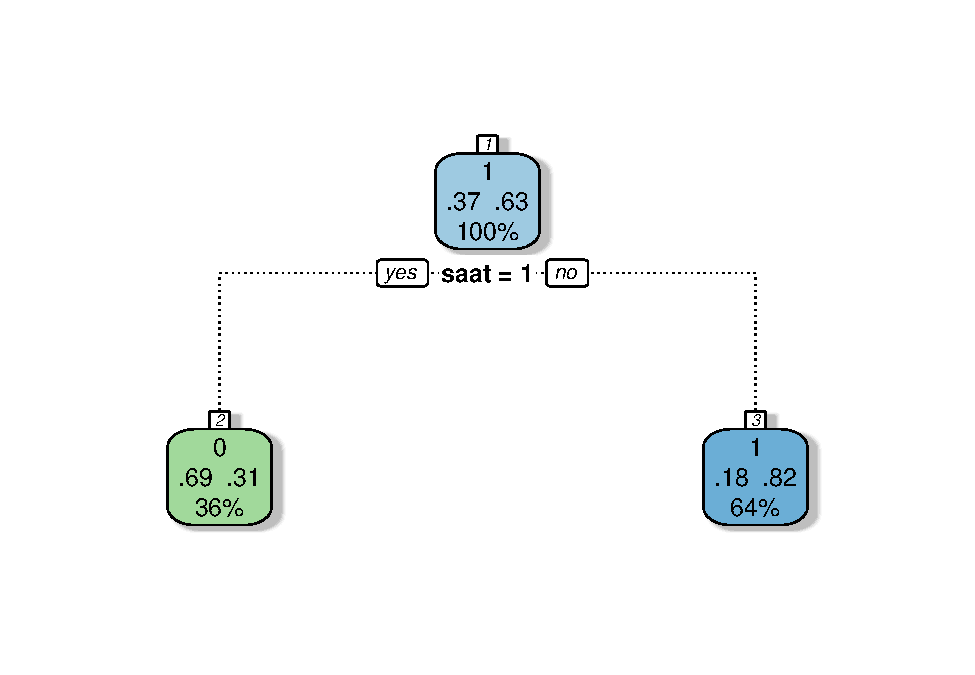
\includegraphics[width=0.76\linewidth]{BP_Rapor_files/figure-latex/unnamed-chunk-25-1} 

}

\caption{CART (En İyi Model)}\label{fig:unnamed-chunk-25}
\end{figure}
CART ağacımız Gini katsayısına göre hesaplanıp, ilk olarak saat kategorik değişkenine ayrılmıştır. Bu durumda OEE'nin yorumlanmasında en önemli değişken olarak saat değişkeni olduğu söylenebilir. Buna göre saati ortalama veya ortalamadan yüksek olanlar, sol tarafa ayrılmıştır. 163 birimlik ``train'' verisi üzerinde hesaplandığı için bu düğüme \%36 oranla 59 birim düşmüştür. 59 birimin \%69'u yani 41 tanesi OEE'si 0 olan sınıfta yer almıştır. Kalan 18 tanesi ise OEE'si 1 olan sınıfta yer almıştır. Saati ortalamadan az olanlar ise, sağ tarafa ayrılmıştır. 163 birimin \%64 oranla 104 birim bu düğüme düşmüştür. 104 birimin \%18'i yani 19 tanesi OEE'si 0 olan sınıfta yer almıştır. Kalan 85 tanesi ise OEE'si 1 olan sınıfta yer almıştır.
\begin{verbatim}
En İyi Model için OEE Karmaşıklık Matrisi 
\end{verbatim}
\begin{verbatim}
          Reference
Prediction  <85  >=85
       <85    5     2
      >=85    3    25
\end{verbatim}
\begin{longtable}[]{@{}lllll@{}}
\toprule
Doğruluk & Kesinlik & Hassaslık & Belirlilik & F1 Skoru\tabularnewline
\midrule
\endhead
0.857 & 0.625 & 0.926 & 0.714 & 0.667\tabularnewline
\bottomrule
\end{longtable}
\hypertarget{yeni-deux11fiux15fken}{%
\subsubsection{Yeni Değişken}\label{yeni-deux11fiux15fken}}

Fabrika verileri ile kurulan lojistik regresyon modelinde saat ve üretim değişkenleri modelde anlamlı çıkmıştır. CART modelinde ise en önemli değişkenin saat olduğu tespit edilmiştir. Daha sonra CART modelinde ağaç derinliği kontrol edildiğinde 2. düğümün üretim değişkenine ayrıldığı gözlemlenmiştir. Fakat üretim değişkeni tek başına yeterli ayrıştırmayı yapamadığından ağaçta kırpılmış olduğu fark edilmiştir.

Modellerde değişken sayısını artırıp modelin nasıl değiştiğini görmek için simülasyon çalışması ile makineyi çalıştıran kişinin tecrübesi (10 yıldan az\&10 yıl ve daha fazla olarak belirlenmiş kategorik değişken) verilerimize eklenmiştir.
Bu yeni değişkene göre yeni modeller kurulmuştur.

\hypertarget{lojistik-regresyon-modeli-tecruxfcbe-uxfcretim-saat-tuxfcs}{%
\subsubsection{Lojistik Regresyon Modeli (Tecrübe, Üretim, Saat (TÜS))}\label{lojistik-regresyon-modeli-tecruxfcbe-uxfcretim-saat-tuxfcs}}
\begin{Shaded}
\begin{Highlighting}[]
\NormalTok{tus.model =}\StringTok{ }\KeywordTok{glm}\NormalTok{(OEE }\OperatorTok{\textasciitilde{}}\NormalTok{tecrube }\OperatorTok{+}\NormalTok{uretim}\OperatorTok{+}\StringTok{ }\NormalTok{saat ,}\DataTypeTok{family=}\NormalTok{binomial, }\DataTypeTok{data=}\NormalTok{train)}
\KeywordTok{summary}\NormalTok{(tus.model)}
\end{Highlighting}
\end{Shaded}
\begin{verbatim}
Call:
glm(formula = OEE ~ tecrube + uretim + saat, family = binomial, 
    data = train)

Deviance Residuals: 
    Min       1Q   Median       3Q      Max  
-2.1667  -0.3807   0.1177   0.5445   1.9852  

Coefficients:
            Estimate Std. Error z value Pr(>|z|)    
(Intercept)  -1.2441     0.4895  -2.541    0.011 *  
tecrube1      2.7232     0.5543   4.913 8.98e-07 ***
uretim1       3.4907     0.7087   4.926 8.41e-07 ***
saat1        -4.0670     0.7303  -5.569 2.56e-08 ***
---
Signif. codes:  0 '***' 0.001 '**' 0.01 '*' 0.05 '.' 0.1 ' ' 1

(Dispersion parameter for binomial family taken to be 1)

    Null deviance: 214.49  on 162  degrees of freedom
Residual deviance: 100.22  on 159  degrees of freedom
AIC: 108.22

Number of Fisher Scoring iterations: 6
\end{verbatim}
Burada en uygun modelde tecrübe, üretim, saat değişkenleri \%95 anlamlılık düzeyinde istatistiksel olarak anlamlı çıkmıştır. Daha sonra OR, CI ve Wald testine bakılmıştır.
\begin{Shaded}
\begin{Highlighting}[]
\KeywordTok{wald.test}\NormalTok{(}\DataTypeTok{b=}\KeywordTok{coef}\NormalTok{(tus.model),}\DataTypeTok{Sigma=}\KeywordTok{vcov}\NormalTok{(tus.model),}\DataTypeTok{Terms=}\DecValTok{1}\OperatorTok{:}\DecValTok{2}\NormalTok{)}
\end{Highlighting}
\end{Shaded}
\begin{verbatim}
Wald test:
----------

Chi-squared test:
X2 = 24.5, df = 2, P(> X2) = 4.8e-06
\end{verbatim}
Kategorik değişkenlerle kurulan lojistik regresyon en iyi modelindeki Wald değerlerine bakıldığında, tüm p değerleri 0.05'den küçük olduğu için katsayılar \%95 güven seviyesinde istatistiksel olarak anlamlı bulunmuştur.
\begin{Shaded}
\begin{Highlighting}[]
\KeywordTok{exp}\NormalTok{(}\KeywordTok{confint}\NormalTok{(tus.model))}
\end{Highlighting}
\end{Shaded}
\begin{verbatim}
Waiting for profiling to be done...
\end{verbatim}
\begin{verbatim}
                  2.5 %       97.5 %
(Intercept) 0.102099647   0.71419154
tecrube1    5.466755363  48.97582068
uretim1     9.408205782 161.53474388
saat1       0.003329586   0.06180391
\end{verbatim}
Ayrıca OR ve güven aralıklarına bakıldığında, OR'a ait güven aralıklarının 1'i içermediği görülmektedir. Bu yüzden OR'ler anlamlıdır ve yorumlanabilir.
\begin{Shaded}
\begin{Highlighting}[]
\KeywordTok{exp}\NormalTok{(}\KeywordTok{coef}\NormalTok{(tus.model))}
\end{Highlighting}
\end{Shaded}
\begin{verbatim}
(Intercept)    tecrube1     uretim1       saat1 
 0.28821447 15.22833475 32.81030772  0.01712815 
\end{verbatim}
10 Yıllık Tecrübesi olanların, olmayanlara göre OEE yüzdesinin yüksek olma şansı yaklaşık olarak 15 kattır. Üretimi yüksek olanların, üretimi düşük olanlara göre OEE yüzdesinin yüksek olma şansı yaklaşık olarak 33 kattır. Saati az olanların saati yüksek olanlara göre OEE yüzdesinin yüksek olma şansı ise 1/0.17 yaklaşık olarak 6 kattır.
\begin{verbatim}
TÜS Model için OEE Karmaşıklık Matrisi 
\end{verbatim}
\begin{verbatim}
          Reference
Prediction  <85  >=85
       <85    5     2
      >=85    3    25
\end{verbatim}
\begin{longtable}[]{@{}lllll@{}}
\toprule
Doğruluk & Kesinlik & Hassaslık & Belirlilik & F1 Skoru\tabularnewline
\midrule
\endhead
0.886 & 0.75 & 0.926 & 0.75 & 0.75\tabularnewline
\bottomrule
\end{longtable}
\hypertarget{cart-algoritmasux131-tecruxfcbe-uxfcretim-saat-tuxfcs}{%
\subsubsection{CART Algoritması (Tecrübe, Üretim, Saat, (TÜS))}\label{cart-algoritmasux131-tecruxfcbe-uxfcretim-saat-tuxfcs}}
\begin{Shaded}
\begin{Highlighting}[]
\NormalTok{cart=}\KeywordTok{rpart}\NormalTok{(}\DataTypeTok{formula =}\NormalTok{ OEE }\OperatorTok{\textasciitilde{}}\StringTok{ }\NormalTok{tecrube }\OperatorTok{+}\NormalTok{uretim}\OperatorTok{+}\StringTok{ }\NormalTok{saat, }\DataTypeTok{data =}\NormalTok{ train, }\DataTypeTok{method =} \StringTok{"class"}\NormalTok{)}
\KeywordTok{fancyRpartPlot}\NormalTok{(cart,}\DataTypeTok{sub =} \StringTok{""}\NormalTok{)}
\end{Highlighting}
\end{Shaded}
\begin{figure}

{\centering 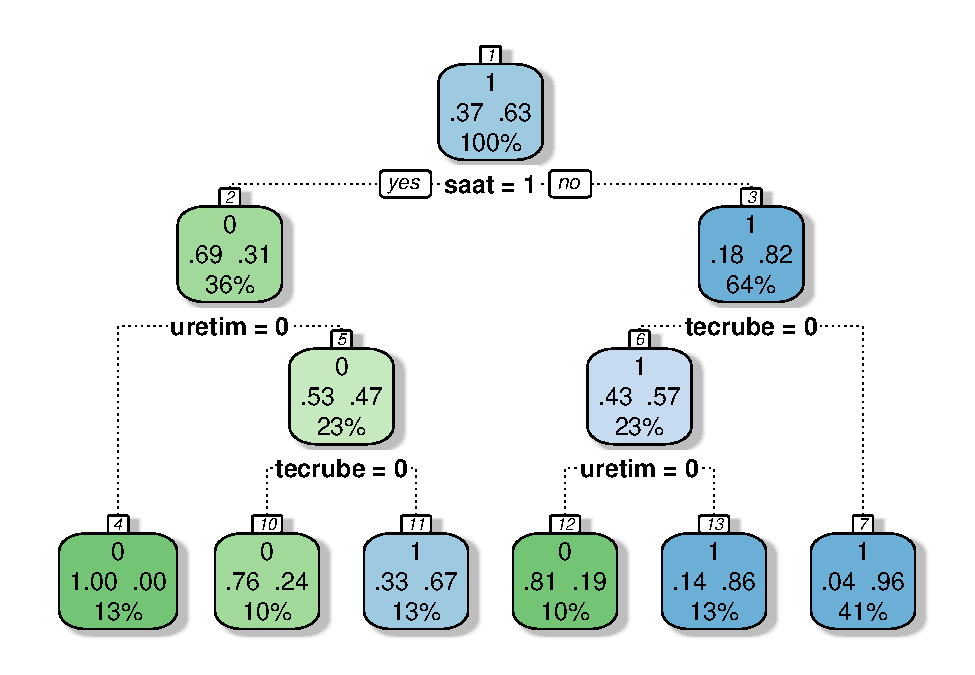
\includegraphics[width=0.8\linewidth]{BP_Rapor_files/figure-latex/unnamed-chunk-35-1} 

}

\caption{CART (TÜS)}\label{fig:unnamed-chunk-35}
\end{figure}
Buna göre saati ortalama veya ortalamadan yüksek olanlar, sol tarafa ayrılıp, 2. Düğümde yer almıştır. 163 birimlik ``train'' verisi üzerinde hesaplandığı için bu 2. düğüme \%36 oranla 59 birim düşmüştür. 59 birimin \%69'u yani 41 tanesi OEE'si 0 olan sınıfta yer almıştır. Kalan 18 tanesi ise OEE'si 1 olan sınıfta yer almıştır.

~2. düğüm daha sonra üretim değişkenine göre ikiye ayrılmıştır. Üretimi ortalama ya da ortalamadan yüksek olanlar sağ tarafa ayrılıp 5. düğümü oluşturmuşlardır. 5. düğüme toplam verinin \%23'üne denk gelen 38 birim düşmüştür. Bu 38 birimin \%53'ü yani 20 tanesi OEE'si 0 olan sınıfta yer almıştır. Kalan 18 tanesi ise OEE'si 1 olan sınıfta yer almıştır.

~2. düğümde üretimi ortalamadan az olanlar sol tarafa ayrılıp 4. düğümü oluşturmuşlardır. 4. düğüme toplam verinin \%13'üne denk gelen 21 birim düşmüştür. Bu 21 birimin \%100'ü yani tamamı OEE'si 0 olan sınıfta yer almıştır. OEE'si 1 olan sınıfta yer alan birim yoktur.

~5. düğüm daha sonra tecrübe değişkenine göre ikiye ayrılmıştır. On yıllık tecrübesi olanlar sol tarafa ayrılıp 10. düğümü, olmayanlar sağ tarafa ayrılıp 11. düğümü oluşturmuşlardır. 10. düğüme toplam verinin \%10'una denk gelen 16 birim düşmüştür. Bu 16 birimin \%76'sı yani 12 tanesi OEE'si 0 olan sınıfta yer almıştır. Kalan 4 tanesi ise OEE'si 1 olan sınıfta yer almıştır.
11. düğüme ise toplam verinin \%13'üne denk gelen 21 birim düşmüştür. Bu 21 birimin \%33'ü yani 7 tanesi OEE'si 0 olan sınıfta yer almıştır. Kalan 14 tanesi ise OEE'si 1 olan sınıfta yer almıştır.

Saati ortalamadan az olanlar ise, sağ tarafa ayrılmıştır. 163 birimin \%64 oranla 104 birim bu düğüme yani 3. düğüme düşmüştür. 104 birimin \%18'i yani 19 tanesi OEE'si 0 olan sınıfta yer almıştır. Kalan 85 tanesi ise OEE'si 1 olan sınıfta yer almıştır.

~3. Düğüm daha sonra tecrübe değişkenine göre ayrılmıştır. On yıllık tecrübesi olmayanlar sol tarafa ayrılıp 6. düğümü oluşturmuştur. 6. düğüme toplam verinin \%23'üne denk gelen 38 birim düşmüştür. Bu 38 birimin \%43'ü yani 16 tanesi OEE'si 0 olan sınıfta yer almıştır. Kalan 22 tanesi ise OEE'si 1 olan sınıfta yer almıştır.

~3. düğümdeki on yıllık tecrübesi olanlar sağ tarafa ayrılıp 7. düğümü oluşturmuşlardır. 7. düğüme toplam verinin \%41'ine denk gelen 67 birim düşmüştür. Bu 67 birimin \%4'ü yani 3 tanesi OEE'si 0 olan sınıfta yer almıştır. Kalan 64 tanesi ise OEE'si 1 olan sınıfta yer almıştır.

~6. düğüm daha sonra üretim değişkenine göre ikiye ayrılmıştır. Üretimi az olanlar sol tarafa ayrılıp 12. düğümü, çok olanlar sağ tarafa ayrılıp 13. düğümü oluşturmuşlardır. 12. düğüme toplam verinin \%10'una denk gelen 16 birim düşmüştür. Bu 16 birimin \%81'i yani 13 tanesi OEE'si 0 olan sınıfta yer almıştır. Kalan 3 tanesi ise OEE'si 1 olan sınıfta yer almıştır. 13. düğüme ise toplam verinin \%13'üne denk gelen 21 birim düşmüştür. Bu 21 birimin \%14'ü yani 3 tanesi OEE'si 0 olan sınıfta yer almıştır. Kalan 18 tanesi ise OEE'si 1 olan sınıfta yer almıştır.
\begin{verbatim}
TÜS Model için OEE Karmaşıklık Matrisi 
\end{verbatim}
\begin{verbatim}
          Reference
Prediction  <85  >=85
       <85    6     2
      >=85    2    25
\end{verbatim}
\begin{longtable}[]{@{}lllll@{}}
\toprule
Doğruluk & Kesinlik & Hassaslık & Belirlilik & F1 Skoru\tabularnewline
\midrule
\endhead
0.886 & 0.75 & 0.926 & 0.75 & 0.75\tabularnewline
\bottomrule
\end{longtable}
\hypertarget{sonuuxe7}{%
\chapter*{Sonuç}\label{sonuuxe7}}
\addcontentsline{toc}{chapter}{Sonuç}

İzmir ili Torbalı ilçesinde plastik masa örtüsü üretimi gerçekleştiren SANEM Plastik A.Ş. adlı fabrikadan 2018-2019 yılları arasında alınan 198 veri ile makine öğrenimi algoritmalarını kullanarak saat ve üretim ve değişkenlerinin OEE puanı üzerindeki etkileri, lojistik regresyon ve CART algoritmaları üzerinden modeller kurulmuştur. Kurulan lojistik regresyon modelinde saat ve üretim değişkenleri modelde anlamlı çıkmıştır. CART modelinde ise en önemli değişkenin üretim olduğu tespit edilmiştir.

Modellerimizin iki büyük kısıtlaması vardır. Biri değişken sayısı diğeri ise örneklem sayısının azlığıdır. Bu amaçla modellemede değişken sayısını artırıp modelin nasıl değiştiğini görmek için verilerimize simülasyon çalışması ile makineyi çalıştıran kişinin tecrübesi(10 yıldan az\&10 yıl ve daha fazla olarak belirlenmiş kategorik değişken) eklenmiştir.

Son eklenen veriler ile lojistik regresyon modelimizde saat, üretim ve tecrübe değişkenlerinin anlamlı, CART modelinde ise en önemli değişkenin üretim olduğu, sonra tecrübe en son olarak da saat olduğu bulunmuştur.

Bu çalışma ile üretim yapan fabrikaların verisinde makine öğrenimi kapsamında yer alan sınıflandırma modellerinden lojistik regresyon ve CART modellerinin uygulanabilirliği tespit edilmiştir. Bu tip verilerde değişik sınıflandırma algoritmaları da kullanılabilir. Ayrıca bu algoritmaların performansları da karşılaştırılabilir.

Fabrikadaki uzmanlarla yapılan ortak çalışmalarla bu tespitin farklı veri türlerinde ve
farklı modellerle yapılması planlanmalıdır. Böylece sanayi-üniversite işbirliği
gerçekleşmesi sağlanabilir.

\backmatter

\hypertarget{kaynaklar}{%
\chapter*{Kaynaklar}\label{kaynaklar}}
\addcontentsline{toc}{chapter}{Kaynaklar}

\markboth{References}{References}

\hypertarget{refs}{}
\begin{cslreferences}
\leavevmode\hypertarget{ref-angel2000}{}%
Angel, E. (2000). \emph{Interactive computer graphics : A top-down approach with opengl}. Boston, MA: Addison Wesley Longman.

\leavevmode\hypertarget{ref-angel2001a}{}%
Angel, E. (2001a). \emph{Batch-file computer graphics : A bottom-up approach with quicktime}. Boston, MA: Wesley Addison Longman.

\leavevmode\hypertarget{ref-angel2001b}{}%
Angel, E. (2001b). \emph{Test second book by angel}. Boston, MA: Wesley Addison Longman.

\leavevmode\hypertarget{ref-wong1999}{}%
Wong, E. (1999). \emph{Artistic Rendering of Portrait Photographs} (Master's thesis). Cornell University.
\end{cslreferences}
\setlength{\parindent}{-0.20in}
\setlength{\leftskip}{0.20in}
\setlength{\parskip}{8pt}

Atalay M., Çelik E., 2017, Artificial İntelligence And Machine Learning Applications İn Big Data Analysis

Özkaya A., 2012, Makine Öğrenmesi İle Ürün Sınıflandırma İncelemesi

KALAYCI E., 2018, Comparison of machine learning techniques for classification of phishing web sites

Abbas G., Shirali M., Moloud V., Amal S., 2018, Predicting the outcome of occupational accidents by CART and CHAID methods at a steel factory in Iran

Yan-yan S., Ying L., 2015, Decision tree methods: applications for classification and prediction

Antipov E., Pokryshevskaya E., 2009, Applying CHAID for logistic regression diagnostics and classification accuracy improvement

\appendix




\end{document}
